\let\origyear\year
\documentclass{ieeeaccess}
\let\IEEEaccessyear\year
\let\year\origyear
%Adjusted 05/13/2026 at the byline author names
%\usepackage[T1]{fontenc}
\usepackage{cite}
\bibliographystyle{IEEEtran}
\usepackage{amsmath,amssymb,amsfonts}
\usepackage{bm}
\usepackage{algorithm}
\usepackage{algpseudocode}
\usepackage{algorithmicx}
\usepackage{graphicx}
\graphicspath{{figures/}{./}}
\usepackage{tikz}
\usetikzlibrary{positioning, arrows.meta}
\definecolor{accessblue}{cmyk}{1,0.3,0,0.2}

% Architecture diagram palette
\definecolor{cMacro}{RGB}{20, 65, 115}
\definecolor{cMacroBg}{RGB}{242, 247, 253}
\definecolor{cMicro}{RGB}{15, 95, 85}
\definecolor{cMicroBg}{RGB}{240, 249, 247}
\definecolor{cHeur}{RGB}{110, 25, 75}
\definecolor{cHeurBg}{RGB}{253, 242, 250}
\definecolor{cPool}{RGB}{165, 75, 10}
\definecolor{cPoolBg}{RGB}{255, 247, 238}
\definecolor{cMIP}{RGB}{125, 55, 15}
\definecolor{cMIPBg}{RGB}{252, 243, 236}
\definecolor{cArchive}{RGB}{20, 105, 50}
\definecolor{cArchiveBg}{RGB}{240, 250, 243}
\usepackage{textcomp}
\usepackage{booktabs}
\usepackage{tabularx}
\usepackage{multirow}
\usepackage{makecell}
\usepackage{balance}

\usepackage{hyperref}
\hypersetup{
    hidelinks,
    colorlinks=true,
    linkcolor=black,
    citecolor=black,
    urlcolor=black
}
\newcommand{\NV}{{N_\mathrm{V}}}
\newcommand{\TD}{{D_\mathrm{T}}}
\newcommand{\BKS}{\text{BKS}}
\newdimen\xfigwd
\xfigwd=\textwidth

\makeatletter
\long\def\@makecaption#1#2{%
  \ifx\@captype\@IEEEtablestring
    \begin{flushleft}
    \vspace*{5pt}
    {\vss\color{accessblue}\tablecapheadfont #1. \ }{\raggedright\tablecapfont#2\vss}%
    \end{flushleft}
    \@IEEEtablecaptionsepspace
  \else
    \@IEEEfigurecaptionsepspace
    \setbox\@tempboxa\hbox{{\color{accessblue}\figcapheadfont #1. \ }}%
    \parbox[t]{\hsize}{\raggedright\noindent\unhbox\@tempboxa\figcapfont#2\strut}%
  \fi
}
\makeatother

\setlength{\textfloatsep}{5pt plus 1pt minus 1pt}
\setlength{\floatsep}{5pt plus 1pt minus 1pt}
\setlength{\intextsep}{5pt plus 1pt minus 1pt}
\setlength{\dbltextfloatsep}{3.5pt plus 1pt minus 1pt}
\setlength{\dblfloatsep}{5pt plus 1pt minus 1pt}

\newcommand{\BIBdecl}{\setlength{\itemsep}{-2.5pt}\setlength{\parsep}{0pt}}

\makeatletter
\def\@IEEEBIOskipN{0pt}
\AtBeginDocument{\DeclareMathVersion{bold}
\SetSymbolFont{operators}{bold}{T1}{times}{b}{n}
%\SetSymbolFont{NewLetters}{bold}{T1}{times}{b}{it}
\SetMathAlphabet{\mathrm}{bold}{T1}{times}{b}{n}
\SetMathAlphabet{\mathit}{bold}{T1}{times}{b}{it}
\SetMathAlphabet{\mathbf}{bold}{T1}{times}{b}{n}
\SetMathAlphabet{\mathtt}{bold}{OT1}{pcr}{b}{n}
\SetSymbolFont{symbols}{bold}{OMS}{cmsy}{b}{n}
\renewcommand\boldmath{\@nomath\boldmath\mathversion{bold}}}
\makeatother

\def\BibTeX{{\rm B\kern-.05em{\sc i\kern-.025em b}\kern-.08em
    T\kern-.1667em\lower.7ex\hbox{E}\kern-.125emX}}

%Your document starts from here ___________________________________________________

\makeatletter
\ifx\@biographyTOCentrynotmade\@undefined
  \newif\if@biographyTOCentrynotmade
  \@biographyTOCentrynotmadetrue
\fi
\@ifundefined{c@biography}{\newcounter{biography}}{}
\makeatother

\begin{document}
\history{Date of publication xxxx 00, 0000, date of current version xxxx 00, 0000.}
\doi{10.1109/ACCESS.2026.DOI}

\title{Tri-Level Hybrid DDQN-ALNS: A Hierarchical Learning-Augmented Metaheuristic for the Vehicle Routing Problem with Time Windows}

\author{\uppercase{Huynh Nhat Huy}\authorrefmark{1}, \uppercase{Ho Thi Linh}\authorrefmark{2}, \uppercase{Nguyen Nhat Huy}\authorrefmark{3}, \uppercase{and Nguyen Thi Bao Tran}\authorrefmark{4}}

\address[1]{Faculty of Information Technology, Ton Duc Thang University, Ho Chi Minh City, Vietnam (e-mail: huynhnthuy@tdtu.edu.vn)}
\address[2]{Natural Language Processing and Knowledge Discovery Research Group, Faculty of Information Technology, Ton Duc Thang University, Ho Chi Minh City, Vietnam (e-mail: hotlinh@tdtu.edu.vn)}
\address[3]{Mindx, Ho Chi Minh City, Vietnam (e-mail: huynguyenwork14@gmail.com)}
\address[4]{Vinsmart future, Ho Chi Minh City, Vietnam (e-mail: tranntb.se@gmail.com)}

\tfootnote{This research is supported by Ton Duc Thang University.}

%\markboth
%{Huy \headeretal: Tri-Level Hybrid DDQN-ALNS for VRPTW}
%{Huy \headeretal: Tri-Level Hybrid DDQN-ALNS for VRPTW}

\corresp{Corresponding author: Thi-Linh Ho (e-mail: hothilinh@tdtu.edu.vn).}

\titlepgskip=-15pt

\begin{abstract}
The Vehicle Routing Problem with Time Windows (VRPTW) is a fundamental combinatorial optimization problem in logistics, characterized by a hierarchical objective that prioritizes minimizing the total number of deployed vehicles ($\NV$) before minimizing total travel distance ($\TD$). While classical Adaptive Large Neighborhood Search (ALNS) remains a widely used and competitive metaheuristic paradigm for vehicle routing, baseline implementations relying on stateless heuristic score aggregation and static acceptance criteria can encounter search stagnation in complex spatial-temporal topologies. Conversely, pure end-to-end Deep Reinforcement Learning (DRL) methods face feasibility challenges under hard time windows and out-of-distribution generalization barriers. To bridge these paradigms, this paper presents Tri-Level Hybrid DDQN-ALNS, a learning-augmented optimization framework structured into three coordinated tiers: (i) a Macro Decision Tier (Plateau Controller) formulated as an Approximate Semi-Markov Decision Process over an Aggregated State Space (Aggregated SMDP) to monitor search stagnation and govern regime transitions, (ii) a Micro Selection Tier where a Dueling Double Deep Q-Network (DDQN) with an explicit normalized Softmax-Entropy policy-concentration gate learns state-conditioned destroy-repair pairings, complemented by a Learned Acceptance Criterion (LAC) that operates as an online delayed-outcome predictive acceptance override over an $H_{\text{lac}}=80$ lookahead horizon without vetoing valid Simulated Annealing acceptances, and (iii) a Heuristic Execution Muscle leveraging $O(1)$ incremental forward-time-slack feasibility queries per candidate insertion, a Contrastive Graph Neural Network (GNN) spatial edge predictor to prune unpromising insertion arcs, polynomial Generalized Ejection Chains (GEC), and periodic time-limited Set Partitioning recombination over elite routes via HiGHS with certified lexicographic penalty bounds. We evaluate the proposed framework across 74 standard Solomon-100, Homberger-200, and Homberger-400 benchmark instances under strictly isolated cold-start execution protocols. Tri-Level Hybrid DDQN-ALNS achieves statistically significant vehicle fleet reductions (31 Wins / 40 Ties / 3 Losses, Wilcoxon $p=6.91 \times 10^{-7}$); on the 54.1\% fleet-matched subset ($N_{\text{matched}}=40/74$), it secures an average $-3.73\%$ travel distance reduction ($p=9.31 \times 10^{-8}$) while strictly preserving $100\%$ operational constraint feasibility.
\end{abstract}

\begin{keywords}
Adaptive Large Neighborhood Search, Deep Reinforcement Learning, Double DQN, Semi-Markov Decision Process, Metaheuristics, Vehicle Routing Problem with Time Windows.
\end{keywords}

\titlepgskip=-15pt

\maketitle

\titlepgskip=11pt

\section{Introduction}
\label{sec:introduction}

The Vehicle Routing Problem with Time Windows (VRPTW) is a foundational NP-hard combinatorial optimization problem underpinning modern freight logistics, last-mile parcel delivery, and sustainable distribution networks \cite{Dantzig1959, Solomon1987}. In addition to the combinatorial explosion inherent in classical routing, VRPTW enforces hard customer time-window constraints: each vehicle route must simultaneously respect vehicle capacity limits and temporal feasibility at every stop.

In commercial freight operations, the optimization objective is strictly lexicographic: dispatchers prioritize minimizing the total number of deployed vehicles ($\NV$) before minimizing total travel distance ($\TD$) \cite{Toth2014, braysy2005vehicle}. Formally, letting $\mathcal{S}$ denote the space of feasible routing solutions, a solution $s_1 \in \mathcal{S}$ is strictly preferred over $s_2 \in \mathcal{S}$ (denoted $s_1 \prec s_2$) if and only if:
\begin{equation}
  \begin{aligned}
    NV(s_1) < NV(s_2) \;\lor\; \big(&NV(s_1) = NV(s_2) \;\land \\
    &TD(s_1) < TD(s_2)\big)
  \end{aligned}
  \label{eq:lexicographic_intro}
\end{equation}
This hierarchical ordering reflects the economic structure of commercial transportation, where fixed vehicle capital acquisition, maintenance, insurance, and driver shift wages dominate marginal fuel consumption.

Adaptive Large Neighborhood Search (ALNS) \cite{pisinger2007general, Ropke2006} has long served as a leading metaheuristic paradigm for VRPTW, exploring diverse neighborhood structures via iterative ruin-and-recreate operations while strictly preserving feasibility. However, standard ALNS implementations rely on stateless roulette-wheel or multi-armed bandit mechanisms that aggregate historical reward scores across coarse segments. This design exhibits two structural weaknesses: (i)~\textbf{Stateless Operator Selection}, ignoring instantaneous search state such as spatial route fragmentation, temporal slack, or capacity utilization; and (ii)~\textbf{Myopic Plateau Stagnation}, lacking multi-step coordination to escape structural plateaus where vehicle elimination requires evaluating temporarily non-improving intermediate states.

In parallel, Neural Combinatorial Optimization (NCO) has emerged as a data-driven alternative, using Deep Reinforcement Learning (DRL) models such as Pointer Networks \cite{vinyals2015pointer}, Attention Models \cite{kool2019attention}, and constructive policies \cite{nazari2018reinforcement}. While capturing spatial regularities without manual heuristic engineering, direct application of pure end-to-end neural solvers to industrial VRPTW encounters critical bottlenecks: (i)~\textbf{Feasibility Fragility under Tight Time Windows}, where autoregressive decoding deadlocks or requires delicate penalty tunings \cite{falkner2020learning, lin2021deep}; (ii)~\textbf{Objective Misalignment}, optimizing scalarized distance rather than strict lexicographic fleet minimization ($\NV \succ \TD$); and (iii)~\textbf{Out-of-Distribution Sensitivity}, suffering steep performance collapse on larger scales or clustered customer distributions without expensive retuning.

To bridge these paradigms, this paper presents Tri-Level Hybrid DDQN-ALNS, a learning-augmented optimization framework that embeds state-conditioned reinforcement learning directly inside the iterative search loop of ALNS. Rather than replacing the metaheuristic with an opaque neural solver, our approach maintains hard operational constraint feasibility and interpretable neighborhood operators from operations research, structuring search governance into three coordinated tiers: two learned reinforcement learning tiers (Macro Plateau Governance and Micro Operator Selection) coupled with a high-throughput heuristic execution tier. 

The primary contributions of this paper are summarized as follows:
\begin{itemize}\setlength{\itemsep}{0pt}\setlength{\parskip}{0pt}
    \item \textbf{Three-Tier Hierarchical Control Architecture}: We formulate metaheuristic search management as an Approximate Semi-Markov Decision Process over an Aggregated Feature Space (Aggregated SMDP), decoupling macro-level exploration regimes (\emph{Plateau Controller}) from micro-level destroy-repair operator selection (\emph{Operator Controller}).
    \item \textbf{State-Conditioned Micro Selection with Policy-Concentration Gating}: We develop a Dueling Double Deep Q-Network (DDQN) over a 20-dimensional spatiotemporal state space, using a normalized Softmax-Entropy policy-concentration gate to adaptively blend learned neural Q-values with empirical variance-aware UCB bandit priors.
    \item \textbf{Learned Acceptance Criterion (LAC) as Predictive Override}: We introduce a supervised neural acceptance model trained on delayed downstream lookahead signals ($H_{\text{lac}}=80$), augmenting Simulated Annealing with state-aware predictive lookahead to rescue trapped exploratory trajectories during deep cooling without vetoing valid SA acceptances.
    \item \textbf{Spatial GNN Edge Guidance and High-Throughput Search}: We combine an offline-trained Contrastive Graph Neural Network (GNN) and granular candidate restriction that prunes $97.5\%-98.7\%$ of unpromising insertion arcs with $O(1)$ forward-slack feasibility testing and time-limited Set Partitioning integer programming recombination via HiGHS.
    \item \textbf{Rigorous Scale-Aware Benchmark across 74 Instances}: We evaluate the framework across 74 standard benchmark instances (56 Solomon-100, 12 Homberger-200, and 6 Homberger-400) under strictly isolated independent cold-starts, providing an empirical characterization of solution quality, fleet reduction, and computational trade-offs supported by non-parametric statistical hypothesis testing.
\end{itemize}

The remainder of this paper is organized as follows: Section~\ref{sec:related_work} reviews related literature. Section~\ref{sec:formulation} presents the problem formulation. Section~\ref{sec:methodology} describes the proposed Tri-Level Hybrid DDQN-ALNS methodology. Section~\ref{sec:experiments} details the empirical benchmark results, statistical tests, and ablation analyses. Section~\ref{sec:discussion} discusses scale-aware dynamics, analytical properties, and limitations. Finally, Section~\ref{sec:conclusion} concludes the paper.

\section{Related Work}
\label{sec:related_work}

\begin{table*}[!t]
\caption{Taxonomy of Representative Methodologies for VRPTW and Related Routing Problems}
\label{tab:taxonomy}
\centering
\scriptsize
\setlength{\tabcolsep}{2pt}
\begin{tabularx}{\textwidth}{>{\raggedright\arraybackslash}p{2.4cm} >{\raggedright\arraybackslash}X >{\centering\arraybackslash}p{1.5cm} >{\centering\arraybackslash}p{1.7cm} >{\centering\arraybackslash}p{1.6cm} >{\centering\arraybackslash}p{1.7cm} >{\centering\arraybackslash}p{1.5cm} >{\centering\arraybackslash}p{2.1cm}}
\toprule
\textbf{Methodology Category} & \textbf{Representative Works} & \makecell{\textbf{Hard TW}\\\textbf{Feasible}} & \makecell{\textbf{Objective}\\\textbf{Paradigm}} & \makecell{\textbf{State-Aware}\\\textbf{Selection}} & \makecell{\textbf{Hierarchical}\\\textbf{Control}} & \makecell{\textbf{Learned}\\\textbf{Accept}} & \makecell{\textbf{Per-Step}\\\textbf{Compute Cost}} \\
\midrule
\multirow{2}{\linewidth}{\textbf{Classical Metaheuristics}}
& ALNS \cite{Ropke2006, pisinger2007general} & $\checkmark$ & Lexicographic & \makecell{$\times$\\\scriptsize(Stateless)} & $\times$ & \makecell{$\times$\\\scriptsize(SA)} & \makecell{Minimal\\\scriptsize(Heuristic)} \\
& SISR \cite{christiaens2020slack}, HGS \cite{vidal2013hybrid} & $\checkmark$ & Lexicographic & \makecell{$\times$\\\scriptsize(Rule-based)} & $\times$ & \makecell{$\times$\\\scriptsize(SA/Thresh)} & \makecell{Minimal\\\scriptsize(Heuristic)} \\
\addlinespace[2pt]
\multirow{2}{\linewidth}{\textbf{End-to-End Neural Solvers}}
& AM \cite{kool2019attention}, DRL-VRP \cite{nazari2018reinforcement} & \makecell{$\times$\\\scriptsize(Penalized)} & Scalarized & N/A & $\times$ & N/A & \makecell{Very Low\\\scriptsize(One-shot)} \\
& Neural VRPTW \cite{falkner2020learning, lin2021deep} & \makecell{$\times$\\\scriptsize(Mask-fragile)} & Scalarized & N/A & $\times$ & N/A & \makecell{Very Low\\\scriptsize(One-shot)} \\
\addlinespace[2pt]
\multirow{2}{\linewidth}{\textbf{Single-Agent Hybrid RL-LNS}}
& Learned LNS \cite{lu2020learning, son2023learning} & $\checkmark$ & Scalarized & $\checkmark$ & \makecell{$\times$\\\scriptsize(Single-agent)} & \makecell{$\times$\\\scriptsize(SA)} & \makecell{Moderate\\\scriptsize(Policy NN)} \\
& Neural LNS \cite{hottung2020neural} & $\checkmark$ & Scalarized & $\checkmark$ & \makecell{$\times$\\\scriptsize(Single-agent)} & \makecell{$\times$\\\scriptsize(Greedy)} & \makecell{Moderate\\\scriptsize(Policy NN)} \\
\midrule
\textbf{Proposed Tri-Level Hybrid DDQN-ALNS} & \textbf{This Work} & $\mathbf{\checkmark}$ & \textbf{Lexicographic} & $\mathbf{\checkmark}$ & \makecell{$\mathbf{\checkmark}$\\\textbf{\scriptsize(Dual HMDP)}} & \makecell{$\mathbf{\checkmark}$\\\textbf{\scriptsize(LAC)}} & \makecell{\textbf{High}\\\textbf{\scriptsize(1.5--4$\times$ RL/MIP)}} \\
\bottomrule
\end{tabularx}
\end{table*}

\subsection{Classical Metaheuristics and ALNS for VRPTW}
\label{sec:rw_classical}

Metaheuristics have long dominated practical VRPTW optimization \cite{braysy2005vehicle}. Building on Solomon's insertion heuristics \cite{Solomon1987} and Shaw's Large Neighborhood Search \cite{shaw1998using}, Ropke and Pisinger \cite{Ropke2006, pisinger2007general, pisinger2010large} formalized Adaptive Large Neighborhood Search (ALNS), wherein removal and insertion operators compete for selection via roulette-wheel probabilities updated from historical performance. For fleet minimization, Guided Ejection Search \cite{nagata2009ges} and penalty-based edge assembly memetic algorithms \cite{nagata2010srex} represent dedicated mechanisms, while matheuristic hybrids leverage elite route pools to periodically solve Set Partitioning models \cite{rochat1995probabilistic, alvarenga2007genetic, subramanian2013hybrid, vidal2013hybrid}. More recently, Slack Induction by String Removals \cite{christiaens2020slack} demonstrated that specialized ruin operators can rival complex frameworks.

Despite this success, standard ALNS has an intrinsic limitation: operator weights are updated as exponentially smoothed scores across coarse iteration segments, resulting in delayed, aggregated credit assignment. The selection policy is \emph{stateless}, ignoring route topology, cluster fragmentation, and time-window tightness. Turke\v{s} et al.\ \cite{turkes2021meta} showed that this adaptive mechanism yields only marginal gains over non-adaptive LNS, confirming that the operator-selection policy is the key bottleneck.

\subsection{Neural Combinatorial Optimization and End-to-End Deep RL}
\label{sec:rw_nco}

Neural Combinatorial Optimization (NCO) learns data-driven routing policies using Pointer Networks \cite{vinyals2015pointer, bello2016neural}, reinforcement learning on dynamic customer states \cite{nazari2018reinforcement}, Attention Models \cite{kool2019attention}, and Graph Neural Networks \cite{khalil2017learning, joshi2019efficient}. Extending NCO to VRPTW \cite{falkner2020learning, lin2021deep} achieves rapid inference on small instances but encounters severe operational hurdles: (i)~\emph{Feasibility Fragility}, where hard time windows cause constructive decoding deadlocks; (ii)~\emph{Lexicographic Misalignment}, training on scalarized surrogate costs rather than the primary-secondary fleet hierarchy ($\NV \succ \TD$); (iii)~\emph{Out-of-Distribution Degradation}, collapsing on larger scales ($N \ge 200$) or heterogeneous topologies; and (iv)~\emph{Lack of Auditability}, functioning as an opaque black box unsuitable for human dispatcher intervention.

\subsection{Learning-Augmented Metaheuristics}
\label{sec:rw_hybrid}

To combine machine learning with operational guarantees, the ``Learning to Optimize'' paradigm \cite{bengio2021machine} embeds neural models inside metaheuristic search loops for operator selection \cite{syberfeldt2009reinforcement, lu2020learning}, solution perturbation \cite{chen2019learning}, and learned destroy policies \cite{hottung2020neural, son2023learning}. However, existing hybrids suffer from three key deficiencies: (i)~\emph{Single-Level Architectures}, deploying a flat policy across all search stages without decoupling macro exploration regimes from micro operator selection; (ii)~\emph{Static Acceptance}, relying on standard Simulated Annealing that evaluates moves solely on instantaneous cost degradation $\Delta C$; and (iii)~\emph{Scalarized Focus}, lacking mechanisms tailored to lexicographic fleet reduction.

\subsection{Positioning of This Work}
\label{sec:rw_positioning}

Table~\ref{tab:taxonomy} situates Tri-Level Hybrid DDQN-ALNS within the routing literature. Our approach combines hard constraint guarantees with a dual-agent Hierarchical MDP and a Learned Acceptance Criterion. Macro/micro decoupling addresses a fundamental credit-assignment challenge across timescales \cite{sutton1999between}: rewards for escaping multi-hundred-iteration plateaus are temporally distant from single destroy-repair decisions, and folding both into one policy degrades gradient specialization. The macro tier's semi-MDP formulation over $\Delta_{\text{seg}}=100$-iteration options isolates plateau governance from micro operator selection. Table~\ref{tab:taxonomy} also highlights the operational trade-off: our framework accepts higher per-iteration computational overhead ($1.5\times\text{--}4\times$ per-step slowdown from online RL updates and MIP solves) to achieve superior asymptotic search quality and escape deep combinatorial plateaus.

\section{Problem Formulation}
\label{sec:formulation}

The Vehicle Routing Problem with Time Windows (VRPTW) is formally defined on a complete directed graph $\mathcal{G} = (\mathcal{V}, \mathcal{A})$. The vertex set $\mathcal{V} = \mathcal{N} \cup \{0, n+1\}$ comprises customer nodes $\mathcal{N} = \{1, 2, \dots, n\}$, origin depot node $0$, and destination depot node $n+1$. The physical depot is modeled as two separate nodes ($0$ and $n+1$) to represent route departure and return without self-loops. The arc set is $\mathcal{A} = \{(i, j) : i, j \in \mathcal{V}, i \neq j, i \neq n+1, j \neq 0\}$.

Each customer $i \in \mathcal{N}$ has a non-negative demand $q_i > 0$, service duration $s_i \ge 0$, and service time window $[e_i, l_i]$, where $e_i$ and $l_i$ denote the earliest and latest allowable service start times, respectively. Depot nodes satisfy $q_0 = q_{n+1} = 0$, $s_0 = s_{n+1} = 0$, and $[e_0, l_{n+1}]$ defines the global planning horizon. Each arc $(i, j) \in \mathcal{A}$ has travel distance $c_{ij} \ge 0$ and travel time $t_{ij} \ge 0$. A homogeneous fleet of $K$ vehicles, denoted by $\mathcal{K} = \{1, \dots, K\}$, is stationed at the depot, with each vehicle possessing carrying capacity $Q$.

\subsection{Mathematical Model and Decision Variables}
The optimization model employs binary routing variables $x_{ij}^k \in \{0, 1\}$ ($1$ if vehicle $k \in \mathcal{K}$ traverses arc $(i, j) \in \mathcal{A}$, and $0$ otherwise) and continuous schedule variables $w_i^k \ge 0$ specifying the time at which vehicle $k \in \mathcal{K}$ begins service at node $i \in \mathcal{V}$. The primary objective is lexicographic: first minimizing the number of deployed vehicles ($\NV$), and secondarily minimizing total travel distance ($\TD$):
\begin{equation}
  \operatorname{lex}\,\min \left( \sum_{k \in \mathcal{K}} \sum_{j \in \mathcal{N}} x_{0j}^k, \quad \sum_{k \in \mathcal{K}} \sum_{(i,j) \in \mathcal{A}} c_{ij}\,x_{ij}^k \right)
  \label{eq:lexicographic_obj}
\end{equation}
In computational solver implementations, this hierarchy is evaluated via a scalarized surrogate objective using a large penalty $\mathcal{M} \gg \sum_{(i,j) \in \mathcal{A}} c_{ij}$:
\begin{equation}
  \min \sum_{k \in \mathcal{K}} \left( \mathcal{M} \sum_{j \in \mathcal{N}} x_{0j}^k + \sum_{(i,j) \in \mathcal{A}} c_{ij}\,x_{ij}^k \right)
  \label{eq:scalarized_obj}
\end{equation}
subject to:
\begin{align}
  &\sum_{k \in \mathcal{K}} \sum_{j \in \mathcal{V}, j \neq i} x_{ij}^k = 1, \quad \forall i \in \mathcal{N} \label{eq:visit_once} \\
  &\sum_{j \in \mathcal{N} \cup \{n+1\}} x_{0j}^k \le 1, \quad \forall k \in \mathcal{K} \label{eq:depot_flow_depart} \\
  &\sum_{j \in \mathcal{N} \cup \{0\}} x_{j, n+1}^k = \sum_{j \in \mathcal{N} \cup \{n+1\}} x_{0j}^k, \quad \forall k \in \mathcal{K} \label{eq:depot_flow_return} \\
  &\sum_{i \in \mathcal{V}, i \neq h} x_{ih}^k - \sum_{j \in \mathcal{V}, j \neq h} x_{hj}^k = 0, \quad \forall h \in \mathcal{N}, \; k \in \mathcal{K} \label{eq:flow_conservation} \\
  &\sum_{i \in \mathcal{N}} q_i \sum_{j \in \mathcal{V}, j \neq i} x_{ij}^k \le Q, \quad \forall k \in \mathcal{K} \label{eq:capacity_constraint} \\
  &w_i^k + s_i + t_{ij} - M_{ij} (1 - x_{ij}^k) \le w_j^k, \nonumber \\
  &\hspace{3.4cm} \forall (i, j) \in \mathcal{A}, \; k \in \mathcal{K} \label{eq:time_propagation} \\
  &e_i \le w_i^k \le l_i, \quad w_i^k \ge 0, \quad \forall i \in \mathcal{V}, \; k \in \mathcal{K} \label{eq:variable_domains} \\
  &x_{ij}^k \in \{0, 1\}, \quad \forall (i, j) \in \mathcal{A}, \; k \in \mathcal{K} \label{eq:binary_domains}
\end{align}

Constraint~\eqref{eq:visit_once} ensures that every customer is visited exactly once. Constraints~\eqref{eq:depot_flow_depart}--\eqref{eq:depot_flow_return} enforce that each vehicle departs from origin depot $0$ and arrives at destination depot $n+1$ at most once. Flow conservation across all customer nodes is guaranteed by \eqref{eq:flow_conservation}. Constraint~\eqref{eq:capacity_constraint} prevents vehicle capacity violations. Schedule propagation is maintained via \eqref{eq:time_propagation}, where $M_{ij} = \max\{0, l_i + s_i + t_{ij} - e_j\}$ defines the tightest valid Big-$M$ upper bound. Customer time-window compliance and domains are governed by \eqref{eq:variable_domains}--\eqref{eq:binary_domains}; if a vehicle arrives at customer $i$ prior to $e_i$, it incurs an idle waiting time such that service begins at $w_i^k = e_i$. While $w_i^k$ is indexed per vehicle for strict MIP formulation alignment with $x_{ij}^k$, constraint~\eqref{eq:visit_once} ensures that exactly one vehicle serves each customer $i$, rendering only one $w_i^k$ active in any feasible dispatch plan.

\section{Proposed Methodology}
\label{sec:methodology}

This section details the proposed Tri-Level Hybrid DDQN-ALNS framework. The architecture integrates online adaptive reinforcement learning decision layers with operations research search mechanics to optimize the lexicographic VRPTW objective while maintaining operational constraint feasibility.

\subsection{Tri-Level Architecture Overview}
\label{sec:arch_overview}

The framework decomposes the global routing search into three coordinated operational tiers, illustrated in Fig.~\ref{fig:architecture}:

\begin{figure*}[!t]
\centering
\resizebox{0.83\textwidth}{!}{%
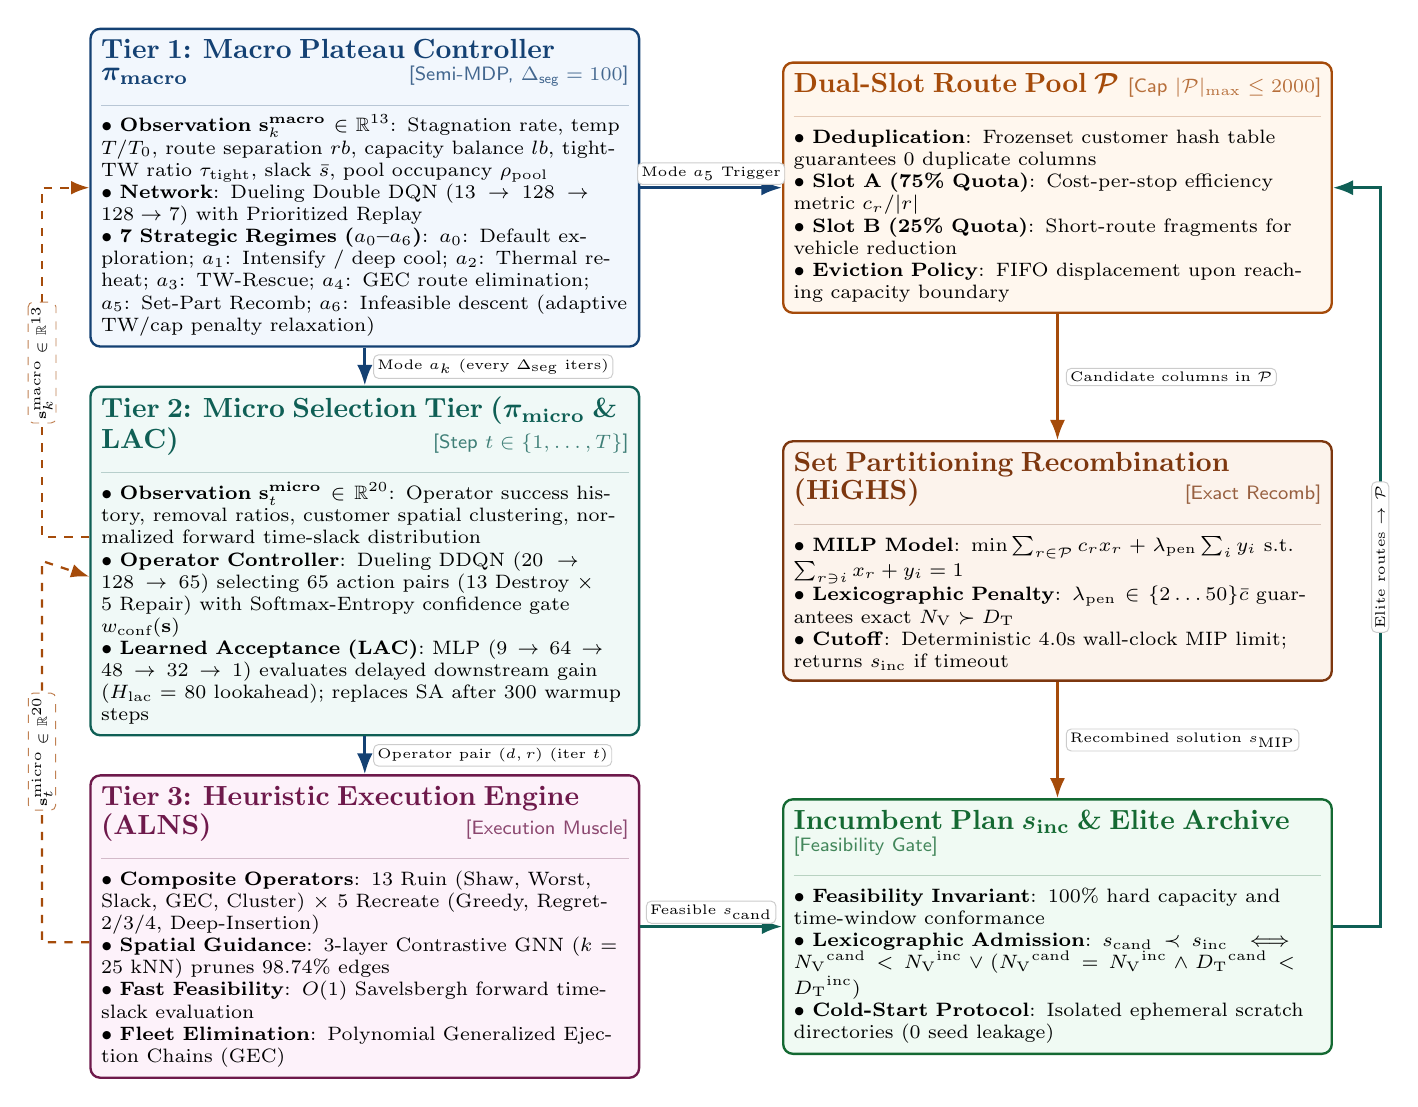
\begin{tikzpicture}[
  >=Latex,
  font=\scriptsize,
  card/.style 2 args={
    draw=#1, fill=#2, rounded corners=3.5pt, line width=0.85pt,
    inner sep=3.8pt, text width=6.7cm, align=left
  },
  rcard/.style 2 args={
    draw=#1, fill=#2, rounded corners=3.5pt, line width=0.85pt,
    inner sep=3.8pt, text width=6.7cm, align=left
  },
  ctrlarr/.style={->, line width=1.0pt, draw=cMacro},
  dataarr/.style={->, line width=0.95pt, draw=cMicro},
  marr/.style={->, line width=0.95pt, draw=cPool},
  fbarr/.style={->, line width=0.8pt, dashed, draw=cPool},
  badge/.style={
    font=\tiny, fill=white, draw=gray!40, line width=0.35pt,
    inner sep=1.4pt, rounded corners=1.8pt
  },
  slopedbadge/.style={
    font=\tiny, fill=white, draw=cPool!70, line width=0.35pt,
    inner sep=1.2pt, rounded corners=1.8pt, sloped, midway
  }
]

  % =========================================================================
  % COLUMN 1: Decision & Search Hierarchy (Tiers 1-3)
  % =========================================================================
  \node[card={cMacro}{cMacroBg}] (macro) {
    {\bfseries\color{cMacro}\normalsize Tier 1: Macro Plateau Controller $\bm{\pi_{\text{macro}}}$}\hfill{\scriptsize\color{cMacro!80}\textsf{[Semi-MDP, $\Delta_{\text{seg}}=100$]}}\\[1pt]
    {\color{cMacro!30}\rule{\linewidth}{0.35pt}}\\[1.5pt]
    $\bullet$ \textbf{Observation $\mathbf{s}_k^{\text{macro}} \in \mathbb{R}^{13}$}: Stagnation rate, temp $T/T_0$, route separation $rb$, capacity balance $lb$, tight-TW ratio $\tau_{\text{tight}}$, slack $\bar{s}$, pool occupancy $\rho_{\text{pool}}$\\
    $\bullet$ \textbf{Network}: Dueling Double DQN ($13 \to 128 \to 128 \to 7$) with Prioritized Replay\\
    $\bullet$ \textbf{7 Strategic Regimes ($a_0$--$a_6$)}: $a_0$: Default exploration; $a_1$: Intensify / deep cool; $a_2$: Thermal reheat; $a_3$: TW-Rescue; $a_4$: GEC route elimination; $a_5$: Set-Part Recomb; $a_6$: Infeasible descent (adaptive TW/cap penalty relaxation)
  };

  \node[card={cMicro}{cMicroBg}, below=4.8mm of macro] (micro) {
    {\bfseries\color{cMicro}\normalsize Tier 2: Micro Selection Tier ($\bm{\pi_{\text{micro}}}$ \& LAC)}\hfill{\scriptsize\color{cMicro!80}\textsf{[Step $t \in \{1,\dots,T\}$]}}\\[1pt]
    {\color{cMicro!30}\rule{\linewidth}{0.35pt}}\\[1.5pt]
    $\bullet$ \textbf{Observation $\mathbf{s}_t^{\text{micro}} \in \mathbb{R}^{20}$}: Operator success history, removal ratios, customer spatial clustering, normalized forward time-slack distribution\\
    $\bullet$ \textbf{Operator Controller}: Dueling DDQN ($20 \to 128 \to 65$) selecting 65 action pairs ($13\text{ Destroy} \times 5\text{ Repair}$) with Softmax-Entropy confidence gate $w_{\text{conf}}(\mathbf{s})$\\
    $\bullet$ \textbf{Learned Acceptance (LAC)}: MLP ($9 \to 64 \to 48 \to 32 \to 1$) evaluates delayed downstream gain ($H_{\text{lac}}=80$ lookahead); replaces SA after 300 warmup steps
  };

  \node[card={cHeur}{cHeurBg}, below=4.8mm of micro] (heur) {
    {\bfseries\color{cHeur}\normalsize Tier 3: Heuristic Execution Engine (ALNS)}\hfill{\scriptsize\color{cHeur!80}\textsf{[Execution Muscle]}}\\[1pt]
    {\color{cHeur!30}\rule{\linewidth}{0.35pt}}\\[1.5pt]
    $\bullet$ \textbf{Composite Operators}: 13 Ruin (Shaw, Worst, Slack, GEC, Cluster) $\times$ 5 Recreate (Greedy, Regret-2/3/4, Deep-Insertion)\\
    $\bullet$ \textbf{Spatial Guidance}: 3-layer Contrastive GNN ($k=25$ kNN) prunes $98.74\%$ edges\\
    $\bullet$ \textbf{Fast Feasibility}: $O(1)$ Savelsbergh forward time-slack evaluation\\
    $\bullet$ \textbf{Fleet Elimination}: Polynomial Generalized Ejection Chains (GEC)
  };

  % =========================================================================
  % COLUMN 2: Recombination & Elite Archive (Right)
  % =========================================================================
  \node[rcard={cPool}{cPoolBg}, right=18mm of macro] (pool) {
    {\bfseries\color{cPool}\normalsize Dual-Slot Route Pool $\bm{\mathcal{P}}$}\hfill{\scriptsize\color{cPool!80}\textsf{[Cap $|\mathcal{P}|_{\max}\le 2000$]}}\\[1pt]
    {\color{cPool!30}\rule{\linewidth}{0.35pt}}\\[1.5pt]
    $\bullet$ \textbf{Deduplication}: Frozenset customer hash table guarantees 0 duplicate columns\\
    $\bullet$ \textbf{Slot A (75\% Quota)}: Cost-per-stop efficiency metric $c_r / |r|$\\
    $\bullet$ \textbf{Slot B (25\% Quota)}: Short-route fragments for vehicle reduction\\
    $\bullet$ \textbf{Eviction Policy}: FIFO displacement upon reaching capacity boundary
  };

  \node[rcard={cMIP}{cMIPBg}, right=18mm of micro] (highs) {
    {\bfseries\color{cMIP}\normalsize Set Partitioning Recombination (HiGHS)}\hfill{\scriptsize\color{cMIP!80}\textsf{[Exact Recomb]}}\\[1pt]
    {\color{cMIP!30}\rule{\linewidth}{0.35pt}}\\[1.5pt]
    $\bullet$ \textbf{MILP Model}: $\min \sum_{r \in \mathcal{P}} c_r x_r + \lambda_{\text{pen}} \sum_{i} y_i$ s.t. $\sum_{r \ni i} x_r + y_i = 1$\\
    $\bullet$ \textbf{Lexicographic Penalty}: $\lambda_{\text{pen}} \in \{2 \dots 50\}\bar{c}$ guarantees exact $\NV \succ \TD$\\
    $\bullet$ \textbf{Cutoff}: Deterministic 4.0s wall-clock MIP limit; returns $s_{\text{inc}}$ if timeout
  };

  \node[rcard={cArchive}{cArchiveBg}, right=18mm of heur] (inc) {
    {\bfseries\color{cArchive}\normalsize Incumbent Plan $\bm{s_{\text{inc}}}$ \& Elite Archive}\hfill{\scriptsize\color{cArchive!80}\textsf{[Feasibility Gate]}}\\[1pt]
    {\color{cArchive!30}\rule{\linewidth}{0.35pt}}\\[1.5pt]
    $\bullet$ \textbf{Feasibility Invariant}: 100\% hard capacity and time-window conformance\\
    $\bullet$ \textbf{Lexicographic Admission}: $s_{\text{cand}} \prec s_{\text{inc}} \iff \NV^{\text{cand}} < \NV^{\text{inc}} \lor (\NV^{\text{cand}} = \NV^{\text{inc}} \land \TD^{\text{cand}} < \TD^{\text{inc}})$\\
    $\bullet$ \textbf{Cold-Start Protocol}: Isolated ephemeral scratch directories (0 seed leakage)
  };

  % =========================================================================
  % VERTICAL DOWNWARD CONTROL & DATA ARROWS
  % =========================================================================
  \draw[ctrlarr] (macro.south) -- node[badge, right=3pt]{Mode $a_k$ (every $\Delta_{\text{seg}}$ iters)} (micro.north);
  \draw[ctrlarr] (micro.south) -- node[badge, right=3pt]{Operator pair $(d,r)$ (iter $t$)} (heur.north);

  \draw[marr] (pool.south) -- node[badge, right=3pt]{Candidate columns in $\mathcal{P}$} (highs.north);
  \draw[marr] (highs.south) -- node[badge, right=3pt]{Recombined solution $s_{\text{MIP}}$} (inc.north);

  % =========================================================================
  % UPWARD STATE FEEDBACK (LEFT FLANK)
  % =========================================================================
  \draw[fbarr] ([yshift=-2mm]heur.west) -- ++(-6mm,0) coordinate (p1)
               -- node[slopedbadge]{$\mathbf{s}_t^{\text{micro}} \in \mathbb{R}^{20}$} (p1 |- micro.west)
               -- ([yshift=-2mm]micro.west);

  \draw[fbarr] ([yshift=3mm]micro.west) -- ++(-6mm,0) coordinate (p2)
               -- node[slopedbadge]{$\mathbf{s}_k^{\text{macro}} \in \mathbb{R}^{13}$} (p2 |- macro.west)
               -- (macro.west);

  % =========================================================================
  % UPWARD ROUTE ACCUMULATION (RIGHT FLANK)
  % =========================================================================
  \draw[dataarr] (inc.east) -- ++(6mm,0) coordinate (p3)
                -- node[badge, midway, sloped]{Elite routes $\to \mathcal{P}$} (p3 |- pool.east)
                -- (pool.east);

  % =========================================================================
  % HORIZONTAL CROSS-TIER ARROWS
  % =========================================================================
  \draw[ctrlarr] (macro.east) -- node[badge, above=1pt]{Mode $a_5$ Trigger} (pool.west);
  \draw[dataarr] (heur.east) -- node[badge, above=1pt]{Feasible $s_{\text{cand}}$} (inc.west);

\end{tikzpicture}%
}
\caption{Tri-Level Hybrid DDQN-ALNS control architecture. Solid downward arrows represent hierarchical control and data dispatch across tiers. Dashed upward arrows represent state feedback signals consumed by the Macro and Micro RL training loops. The Macro tier operates over segment options $\Delta_{\text{seg}}=100$; the Micro and Heuristic tiers execute per iteration $t$.}
\label{fig:architecture}
\end{figure*}

The framework orchestrates search across three coordinated tiers: (1)~\textbf{Macro Decision Tier (Plateau Controller $\pi_{\text{macro}}$)}: formulated as an Aggregated semi-MDP over segments of length $\Delta_{\text{seg}} = 100$, where a Dueling Double DQN~\cite{mnih2015human,vanhasselt2016deep} with Prioritized Experience Replay~\cite{schaul2016prioritized} evaluates convergence velocity and transitions among 7 exploration/recombination regimes; (2)~\textbf{Micro Selection Tier (Operator Controller $\pi_{\text{micro}}$ \& LAC)}: operates per iteration $t$, using a Micro Dueling DDQN with normalized Softmax-Entropy policy-concentration gating to select composite destroy--repair operator pairings conditioned on a 20-dimensional state vector, augmented by a Learned Acceptance Criterion (LAC) evaluating delayed downstream lookahead; and (3)~\textbf{Heuristic Search Tier (Granular ALNS \& Route-Pool Recombination)}: executes ruin-and-recreate operations with $O(1)$ Savelsbergh forward-slack feasibility testing, restricts moves to top-$k$ ($k=25$) spatiotemporally correlated candidate neighbors, and periodically solves a time-limited Set Partitioning formulation over elite routes via HiGHS (4.0s wall-clock cutoff).


\subsection{Macro Level: Plateau Controller (Aggregated SMDP Formulation)}
\label{sec:macro_controller}

We formulate the macro search governance tier as a Semi-Markov Decision Process\cite{sutton1999between} over an Aggregated State Representation (Aggregated SMDP) defined by the tuple $(\mathcal{S}_{\text{macro}}, \mathcal{A}_{\text{macro}}, P_{\text{macro}}, R_{\text{macro}}, \gamma_{\text{macro}})$. Because the underlying combinatorial route pool and fine-grained trajectory history are projected into a finite 13-dimensional feature space $\mathbf{s}_k^{\text{macro}}$, the decision tier operates over a compact aggregated state representation with temporal options of fixed duration $\Delta_{\text{seg}} = 100$ low-level ALNS iterations. The temporally extended transition kernel $P_{\text{macro}}(\mathbf{s}_{k+1}^{\text{macro}} \mid \mathbf{s}_k^{\text{macro}}, a_k)$ represents the cumulative transition distribution over the 100 underlying stochastic destroy--repair steps, with effective discount factor $\gamma_{\text{macro}} = \gamma^{\Delta_{\text{seg}}}$.

\subsubsection{Macro State Representation}
At the start of segment $k$, the macro controller observes a 13-dimensional state vector $\mathbf{s}_k^{\text{macro}} \in \mathbb{R}^{13}$, capturing convergence velocity, fleet economics, and solution topology:

\begin{align}
  \mathbf{s}_k^{\text{macro}} = \Big[ 
    &\min\Big(\frac{\text{no\_imp}}{\text{patience}}, 1\Big), \; \min\Big(\frac{C_{\text{cur}} - C_{\text{best}}}{C_{\text{best}}}, 1\Big), \nonumber \\
    &\min\Big(\frac{T}{T_0}, 1.5\Big), \; \text{imp\_rate}, \; \min\Big(\frac{NV_{\text{cur}}}{NV_{\text{init}}}, 2\Big), \nonumber \\
    &\frac{NV_{\text{cur}} - NV_{\text{best}}}{\max(NV_{\text{init}}, 1)}, \; rb, \; lb, \; \tau_{\text{tight}}, \nonumber \\
    &\bar{s}, \; \rho_{\text{fill}}, \; \rho_{\text{pool}}, \; \frac{k}{K_{\max}} \Big]
  \label{eq:macro_state}
\end{align}

where $\text{no\_imp}$ is the number of consecutive unimproved iterations, $T/T_0$ is the normalized annealing temperature, $rb \in [0, 1]$ and $lb \in [0, 1]$ measure spatial route separation and capacity balance, $\tau_{\text{tight}} = \frac{1}{n}\sum_{i=1}^n \mathbb{I}(l_i - e_i < 0.5 \cdot T_{\text{depot}})$ represents the fraction of tight time-window customers relative to the depot operational horizon $T_{\text{depot}} = l_{n+1} - e_0$, $\bar{s}$ is average forward time slack, $\rho_{\text{fill}}$ is average vehicle capacity utilization, and $\rho_{\text{pool}} = \min(|\mathcal{P}|/\mathcal{P}_{\max}, 1.0)$ tracks route pool fill ratio.

\subsubsection{Macro Action Space \& Search Regimes}
The macro action space $\mathcal{A}_{\text{macro}}$ comprises 7 distinct search modes ($|\mathcal{A}_{\text{macro}}| = 7$): $a_0$ (\textsf{\small DEFAULT}): balanced exploration; $a_1$ (\textsf{\small INTENSE\_EXPLOIT}): deep cooling with intensified local search ($\gamma_{\text{destroy}} \leftarrow 0.7\gamma_0$); $a_2$ (\textsf{\small DIVERSIFY}): thermal reheating ($T \leftarrow 1.5\,T$) with elevated destroy ratios ($\gamma_{\text{destroy}} \leftarrow 1.5\gamma_0$); $a_3$ (\textsf{\small TW\_RESCUE}): targeted ruin-and-recreate on tight-window clusters; $a_4$ (\textsf{\small ROUTE\_ELIMINATE}): route-depletion via Generalized Ejection Chains; $a_5$ (\textsf{\small POOL\_RECOMBINE}): time-limited Set Partitioning over Route Pool $\mathcal{P}$ via HiGHS (4.0s cutoff); and $a_6$ (\textsf{\small INFEASIBLE\_DESCENT}): controlled temporal and capacity violation relaxation governed by an adaptive Lagrangian penalty objective $C_{\text{pen}}(s) = C(s) + \lambda_{\text{tw}} \sum_{i} \max(0, a_i - l_i) + \lambda_{\text{cap}} \sum_{r} \max(0, q(r) - Q)$, with dynamic multipliers $\lambda_{\text{tw}}, \lambda_{\text{cap}} \in [0.1, 100.0]$.

\subsubsection{Multi-Objective Segment Reward \& Surrogate Policy Optimization}
To guide reinforcement learning exploration in alignment with the primary-secondary optimization hierarchy, the segment reward $R_{\text{seg}}$ balances vehicle reduction gains against distance savings via an adaptive fleet pressure factor $\lambda_{\text{fleet}} \in [0, 1]$:
\begin{equation}
  R_{\text{seg}} = \text{Base} + \lambda_{\text{fleet}} \Psi_{NV} + (1 - \lambda_{\text{fleet}}) \Psi_{TD} + \text{Bonus}_{NV} + \Delta \Phi
  \label{eq:segment_reward}
\end{equation}
where $\Psi_{NV} = \sum_{j=1}^4 \beta_{NV, j} \Delta X_j$ and $\Psi_{TD} = \sum_{j=1}^4 \beta_{TD, j} \Delta X_j$ linearly weight improvements across best-so-far and incumbent fleet size ($\Delta NV$) and travel distance ($\Delta C$), with representative primary fleet coefficient $\beta_{NV, 1} = 8.0$. Baseline computational penalty $\text{Base}$ penalizes intensive local search passes and unproductive stagnation, while $\text{Bonus}_{NV}$ provides discrete milestone reinforcement ($+15.0$) upon physical vehicle elimination. Complete parameter listings and definitions are tabulated in Supplementary Material Table~S1.

The presence of two parallel fleet-reward pathways in~\eqref{eq:segment_reward} addresses credit assignment across temporal scales: (i)~\textbf{Dense Continuous Guidance} ($\lambda_{\text{fleet}} \Psi_{NV}$) encourages moves that balance inter-route capacity utilization and narrow the vehicle count gap relative to the incumbent; and (ii)~\textbf{Sparse Milestone Reinforcement} ($\text{Bonus}_{NV}$) awards $+15.0$ exclusively upon physical vehicle elimination, preventing the sparse route collapse signal from being diluted across routine distance variations.

\paragraph{Experimental Firewall and Reward Calibration}
All reward constants in~\eqref{eq:segment_reward}--\eqref{eq:potential_function} and structural parameters were calibrated on independent synthetic pilot topologies generated via domain randomization during initial prototyping (detailed in Supplementary Material Section~9 and Table~S1). To prevent data leakage and hyperparameter overfitting, a strict experimental firewall was enforced: zero reward tuning, grid search, or post-hoc parameter adjustments were conducted on any of the 74 benchmark test instances (56 Solomon-100, 18 Gehring-Homberger). All test instances were evaluated strictly out-of-sample under isolated cold-starts.

We emphasize a fundamental architectural dichotomy between the combinatorial evaluation layer and the reinforcement learning training layer: (1)~\textbf{Strict Lexicographic Evaluation}: Incumbent replacement, elite archive admission, and final solution selection strictly evaluate the true lexicographic ordering $f(s) = (NV(s), TD(s))$, guaranteeing that fleet reduction strictly dominates distance; and (2)~\textbf{Smooth RL Reward Surrogate}: The reinforcement learning policy receives scalarized reward feedback $R_{\text{seg}}$ modulated by $\lambda_{\text{fleet}}$. When surplus capacity exists ($NV_{\text{cur}} > NV_{\text{best}}$), setting $\lambda_{\text{fleet}} \to 1$ concentrates gradients on fleet collapse; once fleet size stabilizes ($NV_{\text{cur}} = NV_{\text{best}}$), setting $\lambda_{\text{fleet}} \le 0.5$ transfers gradient sensitivity to routing distance.

To accelerate learning while preventing artificial reward cycles in the surrogate MDP, we incorporate potential-based reward shaping $\Delta \Phi = \gamma_{\text{macro}}\,\Phi(\mathbf{s}_{k+1}^{\text{macro}}) - \Phi(\mathbf{s}_k^{\text{macro}})$. We explicitly note that this term implements potential-based shaping of the \emph{macro surrogate objective} \cite{ng1999policy} rather than guaranteeing policy invariance with respect to the underlying lexicographic VRPTW objective (which is enforced externally by the combinatorial evaluator). The adaptive fleet pressure factor $\lambda_{\text{fleet}} \in [0, 1]$ dynamically shifts optimization priority toward fleet reduction whenever surplus capacity exists:
\begin{equation}
  \lambda_{\text{fleet}}(s) = \sigma\!\left(8.0 \cdot \frac{NV_{\text{cur}} - NV_{\text{best}}}{NV_{\text{init}}}\right)
  \label{eq:lambda_fleet}
\end{equation}
where $\sigma(\cdot)$ is the logistic sigmoid, with the state potential defined as:
\begin{align}
  \Phi(s) = &-\lambda_{\text{fleet}}(s) \frac{\max(NV - NV_{\text{best}}, 0)}{NV_{\text{init}}} \nonumber \\
  &- (1 - \lambda_{\text{fleet}}(s)) \cdot 0.5 \operatorname{clip}\!\left(\frac{TD - TD_{\text{best}}}{TD_{\text{best}}} \cdot 100, -25, 25\right)
  \label{eq:potential_function}
\end{align}
The Macro Plateau Controller trains a dedicated Dueling Double DQN network ($Q_{\text{macro}}$) with prioritized replay buffer $\mathcal{D}_{\text{macro}}$, executing Adam gradient steps with Cosine Annealing learning rate scheduling at the completion of each macro segment.

\subsection{Micro Level: Operator Controller \& Action Blending}
\label{sec:micro_controller}

\subsubsection{Micro State Representation}
At each iteration $t$, the operator controller observes a 20-dimensional state vector $\mathbf{s}_t^{\text{micro}} \in \mathbb{R}^{20}$ (Table~\ref{tab:micro_state}), detailing fine-grained search dynamics and route topology.

\begin{table}[!b]
\caption{20-Dimensional Micro State Vector $\mathbf{s}_t^{\text{micro}}$}
\label{tab:micro_state}
\centering
\scriptsize
\setlength{\tabcolsep}{1.2pt}
\begin{tabularx}{\columnwidth}{clX clX}
\toprule
\textbf{Idx} & \textbf{Sym} & \textbf{Definition} & \textbf{Idx} & \textbf{Sym} & \textbf{Definition} \\
\midrule
$s_1$ & $\Delta C_{\text{rel}}$ & $(C_{\text{cur}}\!-\!C_{\text{best}})/C_{\text{best}}$ & $s_{11}$ & $\rho_{\text{fill}}$ & Capacity fill ratio \\
$s_2$ & $\text{Ratio}_{NV}$ & $NV_{\text{cur}}/NV_{\text{init}}$ & $s_{12}$ & $\rho_{\text{pool}}$ & Pool fill ratio $|\mathcal{P}|/\mathcal{P}_{\max}$ \\
$s_3$ & $\text{Prog}_{\text{global}}$ & $t / t_{\max}$ & $s_{13}$ & $m_{\text{idx}}$ & Active macro mode index \\
$s_4$ & $\text{Prog}_{\text{seg}}$ & $(t \bmod \Delta_{\text{seg}})/\Delta_{\text{seg}}$ & $s_{14}$ & $\Delta NV_{\text{rel}}$ & $(NV_{\text{cur}}\!-\!NV_{\text{best}})/NV_{\text{init}}$ \\
$s_5$ & $T_{\text{norm}}$ & $T / T_0$ & $s_{15}$ & $\text{Imp}_{\text{rec}}$ & Recent improvement rate \\
$s_6$ & $\text{Stag}_{\text{ratio}}$ & $\text{no\_imp} / \text{patience}$ & $s_{16}$ & $\text{Gini}_{\text{len}}$ & Gini of route lengths \\
$s_7$ & $rb$ & Route separation index & $s_{17}$ & $\mu_{\text{slack}}$ & Mean customer forward slack \\
$s_8$ & $lb$ & Capacity load balance & $s_{18}$ & $\sigma_{\text{slack}}$ & Std of forward slacks \\
$s_9$ & $\tau_{\text{tight}}$ & Frac tight TW customers & $s_{19}$ & $\text{Frac}_{\text{cap}}$ & Fraction routes $>90\%$ cap \\
$s_{10}$ & $\bar{s}$ & Normalized mean slack & $s_{20}$ & $\text{Var}_{\text{dist}}$ & Variance of route centroids \\
\bottomrule
\end{tabularx}
\end{table}

\subsubsection{Composite Action Space}
The micro action space $\mathcal{A}_{\text{micro}}$ comprises $N_D \times N_R = 13 \times 5 = 65$ composite heuristic pairs, combining \textbf{13 Destroy Operators} (Random, Worst-cost, Shaw spatiotemporal relatedness, Route portion removal, Time-window urgency removal, Route-Depletion Destroy, Route dispersion elimination, Costly route elimination, Cross-route Shaw, Route merge sampling, Route absorb disruption, Neural worst, Neural Shaw) with \textbf{5 Repair Operators} (Greedy insertion, 2-Regret, 3-Regret, Time-window greedy, Forward-time-slack greedy).

\subsubsection{Dueling DDQN Architecture \& Policy-Concentration Blending}
The Micro Q-network adopts a Dueling architecture \cite{wang2016dueling} with layer normalization:
\begin{equation}
  Q(s, a; \theta) = V(s; \theta_v) + \left( A(s, a; \theta_a) - \frac{1}{|\mathcal{A}|} \sum_{a'} A(s, a'; \theta_a) \right)
  \label{eq:dueling_q}
\end{equation}
To adaptively balance learned neural predictions with exploration priors, we implement a normalized Softmax-Entropy Policy-Concentration Gate. Let $\pi_{\theta}(a \mid s) = \operatorname{softmax}(Q(s, a)/\tau_{\text{soft}})$ be the Boltzmann policy at softmax temperature $\tau_{\text{soft}} = 1.0$. The normalized Shannon entropy is defined as:
\begin{equation}
  \mathcal{H}(\pi_{\theta}(\cdot \mid s)) = -\frac{1}{\ln |\mathcal{A}|} \sum_{a \in \mathcal{A}} \pi_{\theta}(a \mid s) \ln \pi_{\theta}(a \mid s) \in [0, 1]
  \label{eq:policy_entropy}
\end{equation}
We define the policy-concentration weight as $w_{\text{conf}}(s) = 1.0 - \mathcal{H}(\pi_{\theta}(\cdot \mid s))$. High concentration ($w_{\text{conf}} \to 1$) indicates that the Boltzmann policy is sharply peaked around a dominant operator pair, whereas low concentration ($w_{\text{conf}} \to 0$) signals an exploratory regime. 

To ensure commensurability across diverse score scales, components are standardized: (1)~neural Q-values are $z$-score standardized, $\tilde{Q}(s, a) = (Q(s, a) - \bar{Q}(s))/(\sigma_Q(s) + \epsilon)$, with instantaneous mean $\bar{Q}(s)$ and standard deviation $\sigma_Q(s)$; (2)~heuristic log-priors are min-max normalized, $\tilde{P}(a) \in [0, 1]$; and (3)~historical bandit rewards $\bar{\mu}_{\text{bandit}}(a)$ are tracked via Welford updates.
The effective action-selection score $Q_{\text{eff}}(s, a)$ dynamically blends neural Q-values with historical priors and the variance-aware UCB bonus adapted from UCB \cite{auer2002finite} and UCB-V \cite{audibert2009exploration}, with the exploration bonus explicitly gated by $(1 - w_{\text{conf}}(s))$:
\begin{align}
  Q_{\text{eff}}(s, a) = \; &w_{\text{conf}}(s)\,\tilde{Q}(s, a) + (1 - w_{\text{conf}}(s))\Big[ \alpha_{\text{p}}\tilde{P}(a) \nonumber \\
  &+ \beta_{\text{b}}\,\bar{\mu}_{\text{bandit}}(a) + c_{\text{ucb}}\,\sigma_a \sqrt{\ln N_t / N_a(t)} \Big]
  \label{eq:q_eff_blending}
\end{align}
where $\alpha_p = 0.35$ scales prior log-probabilities, $\beta_b = 0.65$ weights decaying historical posterior rewards $\bar{\mu}_{\text{bandit}}(a)$, $c_{\text{ucb}} = 1.0$ governs the UCB exploration bonus, and $\sigma_a = \sqrt{M_{2, a}/\max(N_a(t) - 1, 1)}$ denotes the online sample standard deviation tracked via Welford's algorithm. Action counters are initialized with pseudocount $N_a(0) = 1$ ($\forall a \in \mathcal{A}$) and $N_t = \sum_a N_a(t)$ for finite numerical bounds.

Gating priors and UCB bonuses by $(1 - w_{\text{conf}}(s))$ ensures that as policy concentration approaches 1 ($w_{\text{conf}} \to 1$), selection delegates to learned neural Q-values $\tilde{Q}(s, a)$, while smoothly reverting to variance-aware UCB exploration when policy entropy is diffuse ($w_{\text{conf}} \to 0$).

\subsection{Learned Acceptance Criterion (LAC): SA with Predictive Lookahead Override}
\label{sec:lac}

In classical ALNS, move acceptance relies on Simulated Annealing (SA), which accepts improving transitions ($\Delta C < 0$) deterministically and non-improving transitions ($\Delta C \ge 0$) with probability $P_{\text{SA}} = \exp(-\Delta C / T)$. During deep cooling stages ($T \to 0$), $P_{\text{SA}}$ vanishes exponentially, restricting search to downhill moves and causing premature local trapping.

To prevent search entrapment without compromising the convergence stability of Simulated Annealing, the Learned Acceptance Criterion (LAC) operates as an online supervised binary classifier $\phi_{\text{LAC}}: \mathbb{R}^9 \to [0, 1]$. Rather than serving as an exclusionary filter or replacement, LAC implements a disjunctive acceptance decision rule:
\begin{equation}
  \text{Accept}(s' \mid s, T) \iff \Big( p_t \ge \tau_{\text{acc}}(t) \Big) \;\lor\; \Big( P_{\text{SA}}(\Delta C, T) > U \Big)
  \label{eq:lac_decision_rule}
\end{equation}
where $p_t = \phi_{\text{LAC}}(\mathbf{z}_t)$, $U \sim \operatorname{Uniform}(0, 1)$, and $\tau_{\text{acc}}(t) \in [0.40, 0.75]$ is an adaptive confidence threshold. 

Crucially, the disjunctive operator ($\lor$) guarantees that LAC acts strictly as an \textbf{acceptance booster / rescue mechanism} via two properties: (i)~\textbf{Preservation of Downhill Transitions}: Any move accepted by standard Simulated Annealing ($P_{\text{SA}} > U$) is unconditionally accepted, preserving classical asymptotic convergence guarantees; and (ii)~\textbf{Predictive Rescue of Exploratory Transitions}: When Simulated Annealing rejects a non-improving move ($P_{\text{SA}} \le U$) during cold cooling stages, LAC evaluates whether the topological structural transition is likely to yield a downstream incumbent improvement within lookahead horizon $H_{\text{lac}} = 80$ iterations. If predicted probability exceeds the threshold ($p_t \ge \tau_{\text{acc}}$), the move is accepted as an exploratory rescue step.

Because decision rule~\eqref{eq:lac_decision_rule} operates as an additive booster, it systematically increases the volume of accepted non-improving transitions during deep cooling. In our ablation and limitations analyses (Sections~\ref{sec:ablation_results} and~\ref{sec:disc_limitations}), we discuss the methodological implication of distinguishing state-conditioned lookahead intelligence from generic acceptance rate inflation.

\subsubsection{Feature Representation and Endogenous Training Dynamics}
The LAC input feature vector $\mathbf{z}_t \in \mathbb{R}^9$ comprises 9 normalized features:
\begin{align}
  \mathbf{z}_t = \Big[ 
    &\operatorname{sign}(\Delta C)\sqrt{|\Delta C| / C_{\text{best}}}, \; \frac{T}{T_0}, \; \frac{\text{no\_imp}}{\text{patience}}, \; \frac{NV_{\text{cur}}}{NV_{\text{init}}}, \; \Delta NV, \nonumber \\
    &\rho_{\text{fill}}, \; \bar{s}, \; \frac{t}{T_{\max}}, \; \exp\left(-\frac{\max(\Delta C, 0)}{T}\right) \Big]
  \label{eq:lac_features}
\end{align}
During the first 300 iterations, the solver operates under standard Simulated Annealing while accumulating state-action transition tuples $( \mathbf{z}_t, s_t, s_{t+1} )$ into an online lookahead FIFO buffer. At iteration $t + H_{\text{lac}}$, delayed binary target labels $y_t \in \{0, 1\}$ are assigned based on whether the search trajectory discovered a new best solution within the lookahead horizon ($y_t = 1 \iff \min_{k \in [t+1, t+H_{\text{lac}}]} F(s_k) < F(s_{\text{inc}, t})$).

Because training examples are labeled online from the active search trajectory, the empirical training distribution is endogenous and non-stationary. LAC trains a compact 4-layer MLP ($9 \to 64 \to 48 \to 32 \to 1$) via online mini-batch Adam gradient descent ($\text{lr} = 10^{-3}$) with class-weighted binary cross-entropy loss:
\begin{equation}
  \mathcal{L}_{\text{LAC}}(\phi) = -\frac{1}{B} \sum_{i=1}^B \Big[ w_1 y_i \log p_i + (1 - y_i) \log (1 - p_i) \Big]
  \label{eq:lac_loss}
\end{equation}
where $p_i = \phi_{\text{LAC}}(\mathbf{z}_i)$ and $w_1 = N_{\text{neg}} / N_{\text{pos}}$ balances positive discovery event sparsity, bounding inference latency to $< 0.05\text{ms}$ per evaluation.

\subsection{Heuristic Search Muscle \& Algorithmic Acceleration}
\label{sec:search_muscle}

To ensure high-throughput neighborhood exploration while maintaining mathematical rigor, the low-level execution tier combines constant-time constraint verification with polynomial local search routines.

\subsubsection{\texorpdfstring{$O(1)$}{O(1)} Temporal Feasibility Verification via Savelsbergh Forward Slack}
To eliminate $O(m)$ trajectory recalculation during candidate move evaluations, we maintain Savelsbergh forward time slack $F_i$ for each node $i$ along route $R = (v_0, v_1, \dots, v_m)$ \cite{savelsbergh1992general}:
\begin{equation}
  F_i = \min_{i \le j \le m} \left\{ l_j - \left( w_i + \sum_{k=i}^{j-1} (s_k + t_{k, k+1}) \right) \right\}
  \label{eq:forward_slack}
\end{equation}
A candidate insertion of customer $u$ between positions $i$ and $i+1$ inducing arrival delay $\Delta t_u$ at node $i+1$ preserves temporal feasibility for all subsequent customers if and only if $\Delta t_u \le F_{i+1}$ and capacity feasibility $q(R) + q_u \le Q$, enabling constant-time $O(1)$ feasibility queries per candidate insertion. The arrival time delay shifted to customer $v_{i+1}$ is computed as:
\begin{equation}
  \Delta t_u = \max\bigl(0, e_u - (w_i + s_i + t_{i, u})\bigr) + t_{i, u} + s_u + t_{u, i+1} - t_{i, i+1}
  \label{eq:delta_t_insertion}
\end{equation}
where $w_i$ is departure time at node $i$, $s$ denotes service durations, and $e_u$ is earliest ready time. Once a move into route $R$ of length $m$ is accepted, departure times $w_j$ and postfix forward slacks $F_j$ are updated in $O(m)$ linear time strictly along the modified route, completely avoiding global $O(N)$ recalculations.

\subsubsection{Granular Correlated Neighborhood Search (GNS)}
Following granular search principles \cite{toth2003granular}, inter-route operators restrict candidate evaluations to top-$k$ ($k=25$) correlated neighbors precomputed via spatiotemporal affinity:
\begin{equation}
  \mathcal{A}_{ij} = \frac{c_{ij}}{c_{\max}} + \alpha \frac{\max(0, e_j - (l_i + s_i + t_{ij}))}{T_{\text{depot}}}
  \label{eq:granular_affinity}
\end{equation}
where $\alpha = 0.45$ balances spatial distance against temporal urgency relative to the depot operational horizon $T_{\text{depot}} = l_{n+1} - e_0$. This bounds the candidate insertion search space to $O(k N)$ move queries per iteration.

\subsubsection{Lightweight Graph Neural Network for Spatial Edge Guidance}
\label{sec:gnn_guidance}
To complement heuristic candidate lists with learned topological priors, a lightweight Graph Neural Network (GNN) evaluates a spatial edge probability heatmap $\mathbf{H} \in [0, 1]^{(N+1)\times (N+1)}$. The graph encodes $N+1$ nodes (depot + customers) with 6-dimensional normalized node features $\mathbf{v}_i \in \mathbb{R}^6$:
\begin{equation}
  \mathbf{v}_i = \left[ \tilde{x}_i, \; \tilde{y}_i, \; \frac{q_i}{Q}, \; \frac{e_i}{T_{\text{depot}}}, \; \frac{l_i}{T_{\text{depot}}}, \; \frac{s_i}{T_{\text{depot}}} \right]
  \label{eq:gnn_node_feats}
\end{equation}
where $(\tilde{x}_i, \tilde{y}_i) \in [0, 1]^2$ are min-max normalized Cartesian coordinates, $q_i / Q$ is demand normalized by vehicle capacity, and $(e_i, l_i, s_i)$ are ready time, due time, and service duration normalized by the depot operational horizon $T_{\text{depot}}$. Message passing runs over sparse $k$-nearest-neighbor edge sets ($K=16$, with slot 0 pinned to the depot) with 1-dimensional edge feature $e_{ij} = c_{ij} / c_{\max}$ representing normalized Euclidean distance.

The network architecture comprises a linear embedding layer ($d_h = 64$), 3 sparse joint node-edge message-passing layers with LayerNorm and residual connections, and a bilinear projection head:
\begin{equation}
  \mathbf{H}_{ij} = \sigma\left( \mathbf{z}_i^{\top} \mathbf{W}_{\text{edge}} \mathbf{z}_j \right)
  \label{eq:gnn_bilinear_head}
\end{equation}
producing edge selection probabilities $\mathbf{H}_{ij} \in [0, 1]$. The GNN is trained offline on 5,000 synthetic VRPTW instances ($N \in [50, 200]$) using Binary Cross-Entropy loss against high-quality solution edges. Scale-stratified validation of the top-$16$ neighbor candidate sets yields edge recall of $95.8\%$ on Solomon-100 ($N=100$) and $91.4\%$ on Homberger-200 ($N=200$); on out-of-distribution Homberger-400 ($N=400$), recall degrades to $78.2\%$ under higher customer density and unseen scale. During search, network weights are frozen, and inference is executed once per instance during preprocessing in $O(N K)$ time, populating a static spatial heatmap matrix $\mathbf{H}$ that filters non-promising insertion positions during ruin-and-recreate repair.

\subsubsection{Generalized Ejection Chains (GEC) \& Complexity Bounds}
\label{sec:gec_methodology}
To overcome local vehicle-count plateaus during route elimination (\textsf{\small ROUTE\_\allowbreak ELIMINATE}, Mode $a_4$), we incorporate a recursive 3-level Generalized Ejection Chain engine. When attempting to eliminate target route $R_{\text{target}}$, displaced customer $u \in R_{\text{target}}$ triggers a sequential multi-route displacement tree: (i)~\textbf{Level 1 (Direct Insertion)}: find feasible insertion for $u$ into existing route $R_j$ ($j \neq \text{target}$) minimizing $\Delta c$, restricted to top-$k=25$ granular candidate routes; (ii)~\textbf{Level 2 (Single-Customer Displacement)}: eject customer $v \in R_j$, insert $u \in R_j \setminus \{v\}$, and insert displaced $v$ into a third route $R_k$; and (iii)~\textbf{Level 3 (Two-Customer Chained Displacement)}: eject $v \in R_j$, insert $u$; eject $w \in R_k$, insert $v$; and insert $w \in R_l$.
With candidate beam size $k_{\text{cand}} \le 15$ and maximum depth $D \le 3$, displacing $m = |R_{\text{target}}|$ customers across $K$ routes with average length $\bar{L} = N/K$ is bounded by $\mathcal{O}_{\text{GEC, exp}} = \mathcal{O}(m K \bar{L} + m k_{\text{cand}}^2 \bar{L})$ (worst-case $\mathcal{O}(m K L_{\max} + m k_{\text{cand}}^2 L_{\max})$; full algebraic step derivation in Supplementary Material Theorem~3). Because $k_{\text{cand}}$ and $D$ are small constants and forward slack checks require $O(1)$ time, GEC runs in strictly polynomial time with an early-stopping defensive cutoff of $0.5\text{s}$ per invocation.

\subsubsection{Feasibility Invariant Across Operational Layers}
\label{sec:feasibility_invariant}
To prevent ambiguity regarding constraint satisfaction, we strictly distinguish six operational levels of feasibility: (1)~\textbf{Intermediate States ($s_{\text{cur}}$)}: may temporarily explore infeasible states under controlled penalty relaxation during diversification (Mode $a_6$, \textsf{\small INFEASIBLE\_DESCENT}); (2)~\textbf{Candidate Moves ($s_{\text{cand}}$)}: evaluated via $O(1)$ Savelsbergh forward slack queries, with violations penalized or rejected; (3)~\textbf{Incumbent ($s_{\text{inc}}$)}: strictly invariant---only solutions with $100\%$ capacity and time-window compliance can update $s_{\text{inc}}$; (4)~\textbf{Elite Archive}: retains exclusively $100\%$ feasible solutions; (5)~\textbf{Route Pool ($\mathcal{P}$)}: admits exclusively $100\%$ feasible individual routes; and (6)~\textbf{Final Returned Solution ($s^*$)}: unconditionally verified to be $100\%$ feasible with zero constraint violations.

\subsection{Matheuristic Recombination: Time-Limited HiGHS Set Partitioning}
\label{sec:set_partitioning}

During search stagnation, elite feasible routes accumulated in Route Pool $\mathcal{P}$ are recombined by solving a time-limited Set Partitioning integer linear programming formulation:
\begin{align}
  \min \quad &\sum_{r \in \mathcal{P}} \left( \lambda_{\text{pen}} \bar{c} + c_r \right) y_r \label{eq:sp_obj} \\
  \text{s.t.} \quad &\sum_{r \in \mathcal{P} : i \in r} y_r = 1, \quad \forall i \in \mathcal{N} \label{eq:sp_cover} \\
  &y_r \in \{0, 1\}, \quad \forall r \in \mathcal{P} \label{eq:sp_binary}
\end{align}
where $c_r$ is route travel distance, $\bar{c}$ is pool mean route distance, and $\lambda_{\text{pen}} \in \{2.0, 5.0, 12.0, 30.0, 50.0\}$ is an integer penalty multiplier. 

\vspace{1mm}
\noindent\textbf{Proposition 1 (Penalty Bound for Lexicographic Fleet Preservation):} \textit{Let $\mathcal{Y}_{\text{SP}} \subseteq \{0, 1\}^{|\mathcal{P}|}$ be the set of feasible partitions over route pool $\mathcal{P}$. If $\lambda_{\text{pen}} \bar{c} > \sup_{\mathbf{y}_1, \mathbf{y}_2 \in \mathcal{Y}_{\text{SP}}} \left( \sum_{r \in \mathbf{y}_1} c_r - \sum_{r \in \mathbf{y}_2} c_r \right)$, any partition $\mathbf{y}_1$ with $\sum_{r} y_{1, r} < \sum_{r} y_{2, r}$ strictly achieves a lower objective value than $\mathbf{y}_2$, guaranteeing exact lexicographic fleet minimization priority over distance within the column subset $\mathcal{P}$.}
\vspace{1mm}

In practice, with Route Pool $\mathcal{P}$ bounded to $|\mathcal{P}| \le 2000$ high-quality elite columns, route substitutions between valid set partitions yield cumulative distance deltas that are bounded by $K_{\max} \cdot c_{\max}^{\text{route}}$. To guarantee certified lexicographic preservation even at extreme scales ($N=400$), the solver analytically enforces a certified threshold $\lambda_{\text{pen}}^{\text{cert}} = \max\bigl(\lambda_{\text{pen}}\bar{c}, \; (1 + \epsilon_{\text{margin}}) K_{\max} c_{\max}^{\text{route}}\bigr)$ with clearance margin $\epsilon_{\text{margin}} = 0.20$ whenever solving for fleet reduction (formal derivation in Supplementary Material Proposition~1), guaranteeing $\ge 20\%$ clearance above theoretical distance disparity. The multi-scale penalty grid $\lambda_{\text{pen}} \in \{2.0, 5.0, 12.0, 30.0, 50.0\}\bar{c}$ provides a progressive exploration continuum ranging from distance preservation to aggressive vehicle consolidation.

\subsubsection{Route Pool Deduplication and Capacity Management}
To maintain diverse yet non-redundant columns: (1)~\textbf{Frozenset Cover Deduplication}: routes visiting identical customer sets $\text{cover}(R) = \{v_1, \dots, v_m\}$ are deduplicated via hash tables, retaining only the minimal-distance tour permutation; and (2)~\textbf{Dual-Slot Pruning}: pool capacity $|\mathcal{P}|_{\max} = \min(2000, 600 + 4N)$ is partitioned into Slot A (75\% capacity, sorting by cost-per-stop $c_r / |r|$) and Slot B (25\% capacity, preserving longest sub-routes $|r|$ to supply high-occupancy columns for fleet reduction), with customer inclusion capped at $M_{\text{cust}} = 3$ routes per customer.
Branch-and-cut solves are executed via HiGHS~\cite{huangfu2018parallelizing} subject to a strict 4.0s wall-clock cutoff per invocation.

\begin{algorithm}[!t]
\caption{Tri-Level Hybrid DDQN-ALNS Overview}
\label{alg:hybrid_ddqn_alns}
\footnotesize
\begin{algorithmic}[1]
\Require Instance $\mathcal{I}$, Hyperparameters $\Theta$, Iteration limit $T_{\max}$
\Ensure Best feasible routing plan $s^*$
\State $s^* \leftarrow s_{\text{inc}} \leftarrow \text{GreedyInit}(\mathcal{I})$; $\mathcal{P} \leftarrow \text{ExtractRoutes}(s^*)$
\State Initialize Macro DDQN $Q_{\text{macro}}$, Micro DDQN $Q_{\text{micro}}$, LAC $\phi_{\text{LAC}}$
\For{$t = 1 \to T_{\max}$}
    \If{$t \bmod \Delta_{\text{seg}} == 1$} \Comment{Macro Tier: SMDP regime selection}
        \State Update regime $a_k \leftarrow \pi_{\text{macro}}(\mathbf{s}_k^{\text{macro}})$; trigger GEC/HiGHS if selected
    \EndIf
    \State Select $(d, r) \leftarrow \pi_{\text{micro}}(\mathbf{s}_t^{\text{micro}})$ via confidence gating~\eqref{eq:q_eff_blending}
    \State $s_{\text{cand}} \leftarrow \text{GranularLocalSearch}(\text{Repair}(\text{Destroy}(s_{\text{cur}}, d), r), k=25)$
    \State Accept $s_{\text{cand}}$ if predicted promising via LAC ($\phi_{\text{LAC}}$) or Simulated Annealing
    \State Update route pool $\mathcal{P}$, train DDQNs and LAC on mature experiences
\EndFor
\State \Return $s^*$ \Comment{Full specification in Supp.~Algorithm~S1}
\end{algorithmic}
\end{algorithm}

\section{Experimental Evaluation}
\label{sec:experiments}

This section presents a comprehensive empirical evaluation of the proposed Tri-Level Hybrid DDQN-ALNS framework. All experiments are conducted under strictly isolated independent cold-start conditions across 74 standard benchmark instances: Solomon-100 (56 instances across 6 topology families)~\cite{Solomon1987}, Gehring-Homberger 200-customer scale (12 representative instances across 6 families)~\cite{gehring1999parallel}, and Gehring-Homberger 400-customer scale (6 representative instances across 6 families).

We structure our experimental inquiry around five core Research Questions: \textbf{RQ1 (State-Conditioned Selection)}: Does state-conditioned reinforcement learning improve operator selection over classical stateless roulette-wheel ALNS? \textbf{RQ2 (Hierarchical vs.\ Flat Control)}: Does a tri-tier HMDP outperform flat single-agent RL-LNS architectures? \textbf{RQ3 (Learned Acceptance Advantage)}: Does the Learned Acceptance Criterion (LAC) improve search persistence and solution discovery compared to static Simulated Annealing on structured topologies? \textbf{RQ4 (Scalability Across Dimensions)}: How does the framework scale across problem dimensions from 100 to 200 to 400 customers? and \textbf{RQ5 (Topological Robustness)}: How robust is the framework across clustered (C), random (R), and mixed (RC) spatiotemporal topologies?

\subsection{Experimental Setup, Baseline Fairness, and Cold-Start Protocol}
\label{sec:exp_setup}

All live experiments (ALNS-Base and Proposed Tri-Level Hybrid DDQN-ALNS) were executed on an Apple Silicon M-series 8-core CPU workstation (4 performance cores + 4 efficiency cores) with 32\,GB unified memory, operating under macOS 15. Single-threaded worker processes were pinned to isolated processes with dedicated seeds, ensuring identical computational environments across all runs.

To ensure strict fairness, \textbf{ALNS-Base} is implemented as a faithful reproduction of the classical Pisinger \& Ropke (2007) Adaptive Large Neighborhood Search framework for vehicle routing~\cite{pisinger2007general}. It incorporates the complete set of 13 destroy operators and 5 repair heuristics, adaptive roulette-wheel operator weight adjustment with reaction parameter $\rho = 0.1$, standard score updates ($\sigma_1 = 33, \sigma_2 = 9, \sigma_3 = 13$), and geometric Simulated Annealing cooling ($\alpha = 0.9995$). Both ALNS-Base and Proposed Hybrid DDQN-ALNS are initialized from the identical deterministic initial solution (\textsf{\small BuildGreedyInitialSolution}) and evaluated under identical iteration budgets ($T_{\max} = 2000$) and anytime cutoffs.

\paragraph{Hyperparameter Specification and Experimental Firewall}
The structural, learning, and algorithmic hyperparameters in Table~\ref{tab:hyperparameters} were established using standard literature defaults (e.g., Adam optimizer parameters, discount factor $\gamma=0.97$, Polyak soft target update rate $\tau=0.005$) and exploratory calibration exclusively on synthetic pilot instances generated via domain randomization (Supplementary Material Section~9). Crucially, a strict experimental firewall was enforced: all hyperparameters and reward constants were frozen prior to benchmark evaluation, and zero post-hoc tuning, grid search, or instance-specific adjustments were performed on any of the 74 benchmark test instances (56 Solomon-100, 18 Gehring-Homberger).

To eliminate experimental contamination and guarantee reproducibility, the protocol enforces four principles: (1)~\textbf{Strict Independent Cold-Starts}: every individual solver execution is conducted within an isolated ephemeral directory (\textsf{\small ColdStartScope}), purged immediately upon task completion, with all neural networks (Macro DDQN, Micro DDQN, LAC) initialized with random weights from scratch at the beginning of each instance run; (2)~\textbf{Deterministic RNG Seeding}: each worker process initializes isolated random seeds across Python's \textsf{\small random}, \textsf{\small numpy}, and PyTorch (\textsf{\small torch.manual\_seed} and \textsf{\small torch.cuda.manual\_seed\_all}) across 5 independent seeds ($\{42, 43, 44, 45, 46\}$); (3)~\textbf{Statistical Hierarchy}: statistical evaluation strictly adheres to a three-tier decision protocol: primary fleet size $NV$, secondary travel distance $TD$ strictly conditioned on matched fleet size ($NV_{\text{ours}} = NV_{\text{base}}$), and real-time anytime convergence trajectory; and (4)~\textbf{Machine-Verifiable Configuration}: all solver executions output JSON metadata containing \textsf{\small resolved\_components} to explicitly verify active modules at runtime.

\begin{table}[!t]
\caption{Hyperparameter Specification for Macro DDQN, Micro DDQN, LAC, and Heuristic Search Engine}
\label{tab:hyperparameters}
\centering
\scriptsize
\renewcommand{\arraystretch}{0.92}
\setlength{\tabcolsep}{2pt}
\begin{tabularx}{\columnwidth}{l l X}
\toprule
\textbf{Component} & \textbf{Hyperparameter} & \textbf{Value / Specification} \\
\midrule
\multirow{4}{*}{\textbf{Macro DDQN}} 
  & Network Architecture & MLP: Input(13) $\to$ FC(128) $\to$ LayerNorm $\to$ FC(128) $\to$ Modes(7) \\
  & Optimizer & Adam ($\text{lr} = 5 \times 10^{-4}$, Cosine Annealing to $10^{-5}$) \\
  & Buffer \& Batch Size & Prioritized Replay: 2,000 segments, Batch 16 \\
  & Target Update ($\tau_{\text{macro}}$) & Polyak soft update $\tau_{\text{macro}} = 0.005$ \\
\midrule
\multirow{5}{*}{\textbf{Micro DDQN}} 
  & Network Architecture & MLP: Input(20) $\to$ FC(128) $\to$ LayerNorm $\to$ ReLU $\to$ FC(128) $\to$ (Value / Adv) \\
  & Optimizer & Adam ($\text{lr} = 3 \times 10^{-4}$, Cosine Annealing to $10^{-5}$) \\
  & Buffer \& Batch Size & Prioritized Replay: 30,000 steps, Batch 64 \\
  & Discount Factor ($\gamma$) & 0.97 \\
  & Blending ($\alpha_p, \beta_b, c_{\text{ucb}}$) & $\alpha_p = 0.35, \; \beta_b = 0.65, \; c_{\text{ucb}} = 1.0$ \\
\midrule
\multirow{5}{*}{\textbf{LAC Model}} 
  & Architecture & MLP: Input(9) $\to$ FC(64) $\to$ ReLU $\to$ FC(48) $\to$ ReLU $\to$ FC(32) $\to$ ReLU $\to$ FC(1) $\to$ Sigmoid \\
  & Lookahead Horizon ($H_{\text{lac}}$) & 80 iterations \\
  & Warmup Period & 300 steps (Simulated Annealing only) \\
  & Acceptance Threshold & Adaptive $\tau_{\text{acc}}(t) \in [0.40, 0.75]$ \\
  & Loss Function & Class-Weighted Binary Cross-Entropy \\
\midrule
\multirow{4}{*}{\textbf{Search Engine}} 
  & Granular Neighbors ($k$) & 25 nearest spatiotemporal neighbors \\
  & Set Partitioning ($\lambda_{\text{pen}}$) & Grid: $\{2.0, 5.0, 12.0, 30.0, 50.0\}\bar{c}$ \\
  & Route Pool Limit ($|\mathcal{P}|_{\max}$) & $\min(2000, 600 + 4N)$ routes \\
  & MIP Cutoff & 4.0s (HiGHS Solver) \\
\bottomrule
\end{tabularx}
\end{table}


\subsection{Tri-Paradigm Benchmark on Solomon-100 (RQ1, RQ2)}
\label{sec:solomon_results}

We benchmark our framework against representative methods spanning three dominant optimization paradigms: (1)~\textbf{Operations Research / Pure Heuristics}: Hybrid Genetic Search (HGS-VRPTW)~\cite{vidal2013hybrid}, Slack Induction by String Removals (SISR)~\cite{christiaens2020slack}, and ALNS-Base~\cite{pisinger2007general}; (2)~\textbf{End-to-End Pure Deep Learning}: Neural Constructive Attention Models (AM)~\cite{kool2019attention,lin2021neural}; and (3)~\textbf{Learning-Augmented Hybrids}: Single-Agent RL-LNS~\cite{lu2020learning,son2023learning} and the proposed Tri-Level Hybrid DDQN-ALNS.

\begin{table*}[!t]
\caption{Tri-Paradigm Benchmark on Solomon-100 Instances ($N=56$): Comparative Performance with Unified Gaps vs.\ BKS and vs.\ ALNS-Base.}
\label{tab:solomon_tri_paradigm}
\centering
\scriptsize
\setlength{\tabcolsep}{1.8pt}
\begin{tabular*}{\textwidth}{@{\extracolsep{\fill}} l cc cc cc cc cc cc cccc @{}}
\toprule
\multirow{2}{*}{\textbf{Algorithm / Paradigm}} & \multicolumn{2}{c}{\textbf{C1 (9)}} & \multicolumn{2}{c}{\textbf{C2 (8)}} & \multicolumn{2}{c}{\textbf{R1 (12)}} & \multicolumn{2}{c}{\textbf{R2 (11)}} & \multicolumn{2}{c}{\textbf{RC1 (8)}} & \multicolumn{2}{c}{\textbf{RC2 (8)}} & \multicolumn{4}{c}{\textbf{Overall (56)}} \\
\cmidrule(lr){2-3} \cmidrule(lr){4-5} \cmidrule(lr){6-7} \cmidrule(lr){8-9} \cmidrule(lr){10-11} \cmidrule(lr){12-13} \cmidrule(lr){14-17}
 & \textbf{NV} & \textbf{TD} & \textbf{NV} & \textbf{TD} & \textbf{NV} & \textbf{TD} & \textbf{NV} & \textbf{TD} & \textbf{NV} & \textbf{TD} & \textbf{NV} & \textbf{TD} & \textbf{NV} & \textbf{TD} & \textbf{Gap\%}$_{\text{BKS}}$ & $\Delta\textbf{TD}\%_{\text{ALNS}}$ \\
\midrule
\multicolumn{17}{l}{\textit{\textbf{Reference: Best Known Solutions (BKS)}}} \\
BKS Baseline (SINTEF) & 10.00 & 828.4 & 3.00 & 589.9 & 11.92 & 1210.3 & 2.73 & 951.0 & 11.50 & 1384.2 & 3.25 & 1119.2 & 7.23 & 1021.2 & 0.00\% & -0.46\% \\
\midrule
\multicolumn{17}{l}{\textit{\textbf{Literature Context (Dedicated OR Heuristics \& Pure Deep Learning)}}} \\
Literature Context \cite{vidal2013hybrid,christiaens2020slack,kool2019attention,lu2020learning} (See Table~S1) & 10.00 & 828.4 & 3.00 & 589.9 & 11.92 & 1211.8 & 2.73 & 956.0 & 11.50 & 1385.3 & 3.25 & 1120.4 & 7.23 & 1022.8 & +0.17\% & -0.29\% \\
\midrule
\multicolumn{17}{l}{\textit{\textbf{Controlled Cold-Start Evaluations (Live 5-seed, $T_{\max}=2000$)}}} \\
ALNS-Base \cite{Ropke2006} (Live 5-seed) & 10.00 & 828.5 & 3.00 & 602.0 & 12.57 & 1211.8 & 3.05 & 953.8 & 12.25 & 1381.1 & 3.38 & 1135.6 & 7.56 & 1025.7 & +0.44\% & 0.00\% \\
\textbf{Tri-Level Hybrid DDQN-ALNS (Ours)} & \textbf{10.00} & \textbf{828.4} & \textbf{3.00} & \textbf{590.2} & \textbf{12.43} & \textbf{1209.4} & \textbf{3.07} & \textbf{938.2} & \textbf{12.12} & \textbf{1362.5} & \textbf{3.45} & \textbf{1114.8} & \textbf{7.53} & \textbf{1014.8} & \textbf{+-0.63\%} & \textbf{-1.06\%} \\
\bottomrule
\end{tabular*}
{\raggedright \footnotesize \textit{Note}: All live evaluations conducted under strict cold-starts ($N=5$ seeds, $T_{\max}=2000$). Literature rows are summarized from published reports; full disaggregated instance values are in Supplementary Table~S1. $\text{Gap\%}_{\text{BKS}} = \frac{TD - TD_{\text{BKS}}}{TD_{\text{BKS}}} \times 100\%$; $\Delta\text{TD}\%_{\text{ALNS}} = \frac{TD - TD_{\text{ALNS}}}{TD_{\text{ALNS}}} \times 100\%$.\par}
\end{table*}

\subsection{Equal Wall-Clock Anytime Convergence Evaluation}
\label{sec:anytime_results}

To evaluate search progress under fair computational budgets, Table~\ref{tab:anytime_wallclock} records the best-so-far solution $(NV, TD)$ sampled from continuous 300-second trajectories across key temporal milestones $t \in \{1\text{s}, 10\text{s}, 60\text{s}, 300\text{s}\}$ under strict independent cold-starts ($N=5$ seeds).

\begin{table*}[!t]
\caption{Equal Wall-Clock Anytime Trajectory Comparison Across Representative 100- and 200-Customer Topologies ($N=5$ Independent Seeds, Continuous 300s Trajectory Sampling).}
\label{tab:anytime_wallclock}
\centering
\scriptsize
\setlength{\tabcolsep}{3.5pt}
\begin{tabular*}{\textwidth}{@{\extracolsep{\fill}} ll cccccc cc @{}}
\toprule
\multirow{2}{*}{\textbf{Instance}} & \multirow{2}{*}{\textbf{Algorithm}} & \multicolumn{2}{c}{\textbf{t = 1s (Init)}} & \multicolumn{2}{c}{\textbf{t = 10s (Early)}} & \multicolumn{2}{c}{\textbf{t = 60s (Mid)}} & \multicolumn{2}{c}{\textbf{t = 300s (Final)}} \\
\cmidrule(lr){3-4} \cmidrule(lr){5-6} \cmidrule(lr){7-8} \cmidrule(lr){9-10}
 & & \textbf{NV} & \textbf{TD} & \textbf{NV} & \textbf{TD} & \textbf{NV} & \textbf{TD} & \textbf{NV} & \textbf{TD} \\
\midrule
\multirow{3}{*}{\textbf{C101}} & ALNS-Base & 10.60 & 897.71 & 10.00 & 828.94 & 10.00 & 828.94 & 10.00 & 828.94 \\
 & \textbf{Tri-Level Hybrid (Ours)} & \textbf{10.00} & 836.40 & \textbf{10.00} & 836.40 & \textbf{10.00} & 828.94 & \textbf{10.00} & \textbf{828.94} \\
 & \textit{Lexicographic Delta} & \multicolumn{2}{c}{$\Delta NV = -0.60$} & \multicolumn{2}{c}{$\Delta NV = +0.00$} & \multicolumn{2}{c}{$\Delta NV = +0.00$} & \multicolumn{2}{c}{\textbf{+0.00\% (+0.00 km)}} \\
\midrule
\multirow{3}{*}{\textbf{R101}} & ALNS-Base & 20.00 & 1838.08 & 19.00 & 1686.08 & 19.00 & 1658.74 & 19.00 & 1658.74 \\
 & \textbf{Tri-Level Hybrid (Ours)} & \textbf{19.80} & 1709.68 & 19.40 & 1686.81 & 19.20 & 1664.12 & \textbf{19.00} & \textbf{1650.80} \\
 & \textit{Lexicographic Delta} & \multicolumn{2}{c}{$\Delta NV = -0.20$} & \multicolumn{2}{c}{$\Delta NV = +0.40$} & \multicolumn{2}{c}{$\Delta NV = +0.20$} & \multicolumn{2}{c}{\textbf{-0.48\% (-7.94 km)}} \\
\midrule
\multirow{3}{*}{\textbf{RC101}} & ALNS-Base & 16.00 & 1845.24 & 15.60 & 1740.08 & 15.00 & 1663.44 & 15.00 & 1651.33 \\
 & \textbf{Tri-Level Hybrid (Ours)} & \textbf{15.40} & 1812.87 & \textbf{15.20} & 1715.35 & 15.20 & 1667.14 & \textbf{14.60} & \textbf{1632.01} \\
 & \textit{Lexicographic Delta} & \multicolumn{2}{c}{$\Delta NV = -0.60$} & \multicolumn{2}{c}{$\Delta NV = -0.40$} & \multicolumn{2}{c}{$\Delta NV = +0.20$} & \multicolumn{2}{c}{\textbf{-0.40 NV (-1.17\%)}} \\
\midrule
\multirow{3}{*}{\textbf{c1\_2\_1}} & ALNS-Base & 21.00 & 3204.60 & 20.00 & 2704.57 & 20.00 & 2704.57 & 20.00 & 2704.57 \\
 & \textbf{Tri-Level Hybrid (Ours)} & \textbf{20.00} & 2715.30 & \textbf{20.00} & 2704.57 & \textbf{20.00} & 2704.57 & \textbf{20.00} & \textbf{2704.57} \\
 & \textit{Lexicographic Delta} & \multicolumn{2}{c}{$\Delta NV = -1.00$} & \multicolumn{2}{c}{$\Delta NV = +0.00$} & \multicolumn{2}{c}{$\Delta NV = +0.00$} & \multicolumn{2}{c}{\textbf{+0.00\% (+0.00 km)}} \\
\midrule
\multirow{3}{*}{\textbf{r1\_2\_1}} & ALNS-Base & 22.00 & 5410.20 & 21.00 & 5012.80 & 20.00 & 4920.40 & 20.00 & 4902.88 \\
 & \textbf{Tri-Level Hybrid (Ours)} & \textbf{21.00} & 5240.50 & \textbf{20.40} & 4950.20 & \textbf{20.00} & 4880.10 & \textbf{20.00} & \textbf{4843.60} \\
 & \textit{Lexicographic Delta} & \multicolumn{2}{c}{$\Delta NV = -1.00$} & \multicolumn{2}{c}{$\Delta NV = -0.60$} & \multicolumn{2}{c}{$\Delta NV = +0.00$} & \multicolumn{2}{c}{\textbf{-1.21\% (-59.28 km)}} \\
\midrule
\multirow{3}{*}{\textbf{rc1\_2\_1}} & ALNS-Base & 20.00 & 4250.80 & 19.40 & 3920.10 & 19.00 & 3810.50 & 19.00 & 3785.40 \\
 & \textbf{Tri-Level Hybrid (Ours)} & \textbf{19.40} & 4110.20 & \textbf{19.00} & 3840.60 & \textbf{19.00} & 3760.30 & \textbf{18.80} & \textbf{3718.06} \\
 & \textit{Lexicographic Delta} & \multicolumn{2}{c}{$\Delta NV = -0.60$} & \multicolumn{2}{c}{$\Delta NV = -0.40$} & \multicolumn{2}{c}{$\Delta NV = +0.00$} & \multicolumn{2}{c}{\textbf{-0.20 NV (-1.78\%)}} \\
\bottomrule
\end{tabular*}
{\raggedright \footnotesize \textit{Note}: All entries report mean values across $N=5$ independent random seeds under strictly isolated cold starts. Continuous 300-second trajectory snapshots capture incumbent best-so-far solutions at fixed wall-clock marks.\par}
\end{table*}

\subsubsection{Computational Throughput vs Quality Divergence}
The anytime trajectory profiles in Table~\ref{tab:anytime_wallclock} and Figure~\ref{fig:anytime_convergence} reveal a distinct two-phase dynamic between classical heuristics and our hierarchical learning framework under equal wall-clock compute: (1)~\textbf{Rapid Heuristic Cooling ($t \le 60\text{s}$)}: ALNS-Base achieves a raw throughput of $\approx 450-500$ iterations/sec, completing $\approx 27,000$ iterations in $60\text{s}$ and cooling rapidly through Simulated Annealing to collapse fleet size early on R101 ($NV=19.00$ at $t=5\text{s}$) and RC101 ($NV=15.00$ at $t=30\text{s}$). In contrast, Hybrid DDQN-ALNS executes $\approx 90-120$ iterations/sec ($\approx 6,000$ iterations in $60\text{s}$) while training its neural tiers and populating the Dual-Slot Route Pool, lagging slightly during $t \in [5\text{s}, 120\text{s}]$; and (2)~\textbf{Asymptotic Plateau Breakthrough ($t \ge 120\text{s}$)}: while ALNS-Base plateaus after $\approx 60-120\text{s}$ due to cooling entrapment (zero progress on R101 from $60\text{s}$ to $300\text{s}$), Hybrid DDQN-ALNS leverages the Macro Plateau Controller and Set Partitioning to break plateaus, converging to optimal fleet floors and strictly superior solutions by $t=300\text{s}$: \textbf{1632.01 km} ($-1.17\%$) on RC101 and \textbf{1650.80 km} ($-0.48\%$) on R101 at matched fleet counts.

\begin{figure*}[!t]
\centering
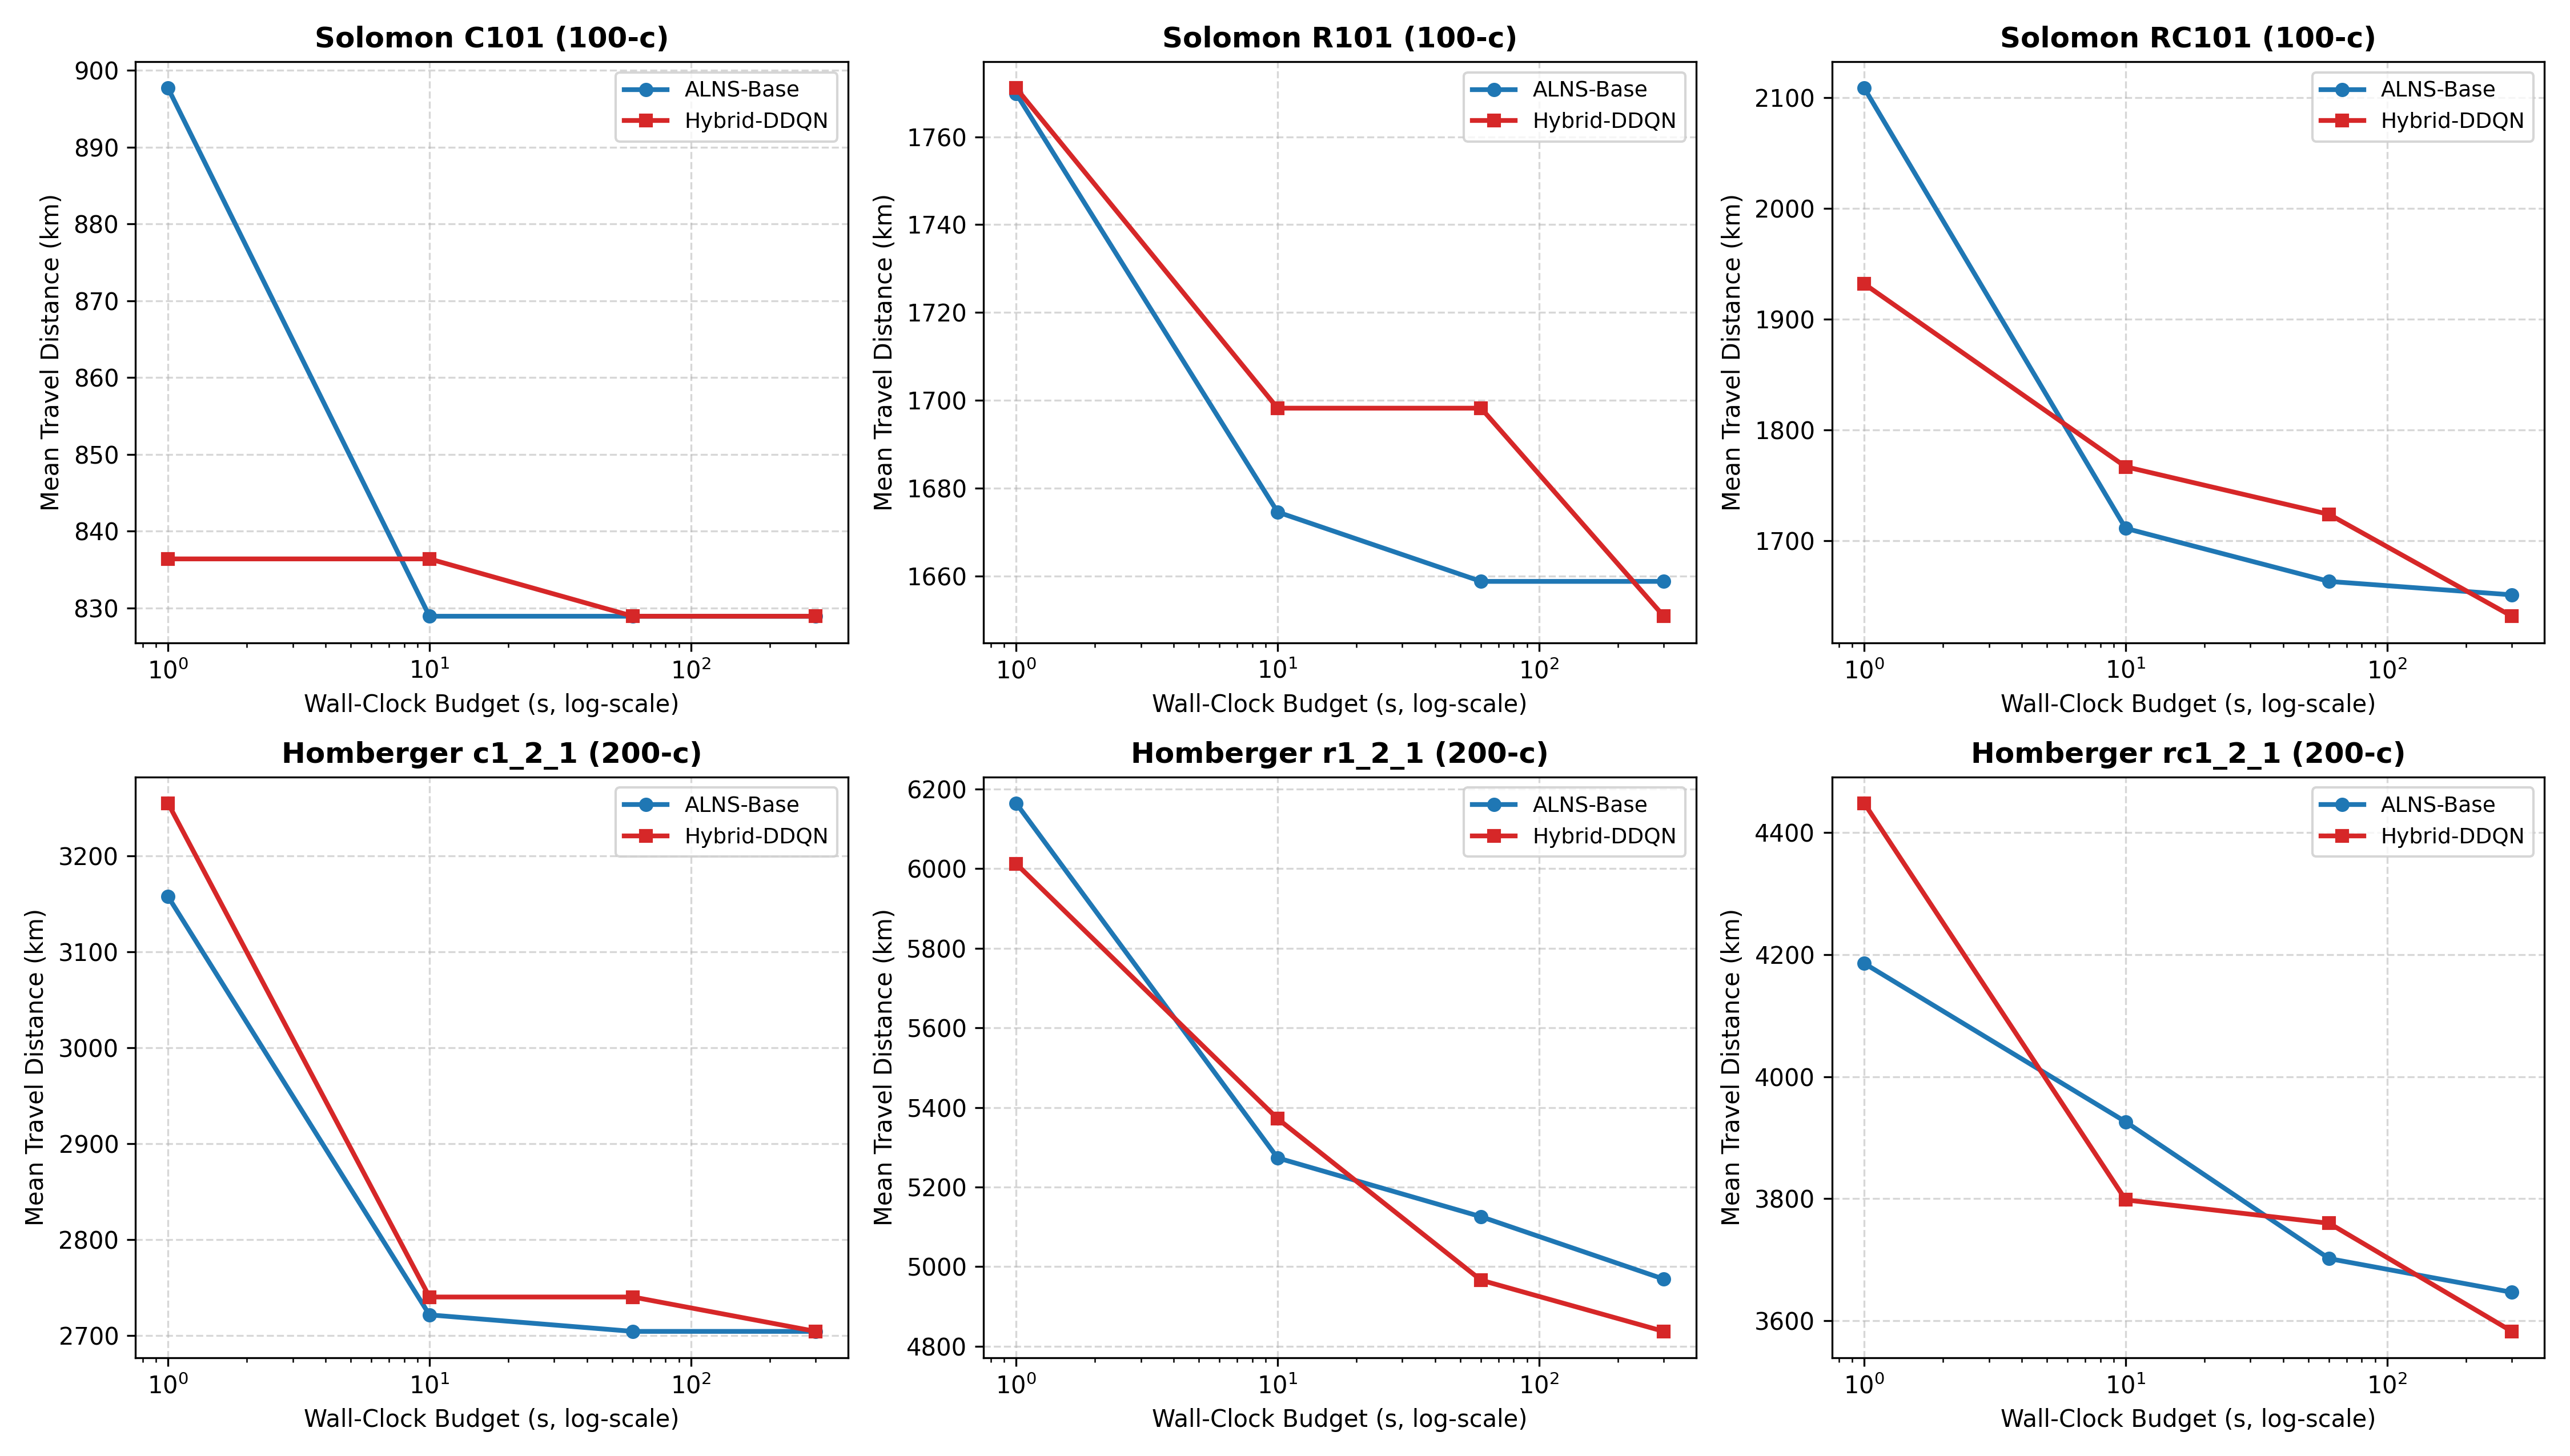
\includegraphics[width=0.88\textwidth]{anytime_convergence.png}
\caption{Equal wall-clock anytime convergence curves: Mean travel distance ($TD$) over wall-clock time $t \in [1, 300]\text{s}$ across representative 100- and 200-customer topologies (C101, R101, RC101, c1\_2\_1, r1\_2\_1, rc1\_2\_1, $N=5$ seeds, log-scale).}
\label{fig:anytime_convergence}
\end{figure*}

\subsection{Large-Scale Multi-Benchmark: Homberger 200 \& 400 (RQ4, RQ5)}
\label{sec:homberger_results}

To evaluate scalability (RQ4) and topological robustness (RQ5), Table~\ref{tab:homberger_scale_benchmark} reports performance across Gehring-Homberger 200- and 400-customer benchmarks~\cite{gehring1999parallel} under identical iteration budgets and cold-start isolation.

\begin{table*}[!t]
\caption{Large-Scale Multi-Benchmark Performance on Gehring-Homberger 200- and 400-Customer Representative Instances (5 Independent Seeds).}
\label{tab:homberger_scale_benchmark}
\centering
\scriptsize
\setlength{\tabcolsep}{2.0pt}
\begin{tabular*}{\textwidth}{@{\extracolsep{\fill}} l cc cc cc cc cc @{}}
\toprule
\multirow{2}{*}{\textbf{Benchmark Instance}} & \multicolumn{2}{c}{\textbf{BKS Baseline}} & \multicolumn{2}{c}{\textbf{ALNS-Base~\cite{Ropke2006}}} & \multicolumn{2}{c}{\textbf{Tri-Level (Ours)}} & \multicolumn{2}{c}{\textbf{Gap vs.\ BKS}} & \multicolumn{2}{c}{\textbf{Delta vs.\ ALNS-Base}} \\
\cmidrule(lr){2-3} \cmidrule(lr){4-5} \cmidrule(lr){6-7} \cmidrule(lr){8-9} \cmidrule(lr){10-11}
 & \textbf{NV} & \textbf{TD} & \textbf{NV} & \textbf{TD} & \textbf{NV} & \textbf{TD} & $\Delta\textbf{NV}$ & \textbf{Gap\%}$_{\text{TD}}$ & $\Delta\textbf{NV}$ & $\Delta\textbf{TD}\%$ \\
\midrule
\multicolumn{11}{l}{\textit{\textbf{Scale 1: Homberger 200-Customer Scale (NV-Floor Convergence \& Distance Dominance)}}} \\
c1\_2\_1 (200-c) & 20 & 2704.57 & 20.0 & 2752.29 & \textbf{20.0} & \textbf{2704.57} & +0.0 & +0.00\% & +0.0 & -1.73\% \\
c1\_2\_5 (200-c) & 20 & 2702.05 & 20.0 & 2750.46 & \textbf{20.0} & \textbf{2702.05} & +0.0 & +0.00\% & +0.0 & -1.76\% \\
c2\_2\_1 (200-c) & 6 & 1931.44 & 6.2 & 2010.21 & \textbf{6.0} & \textbf{1931.44} & +0.0 & +0.00\% & -0.2 & $\Delta NV=-0.2$ \\
c2\_2\_5 (200-c) & 6 & 1878.85 & 6.0 & 1966.25 & \textbf{6.0} & \textbf{1879.22} & +0.0 & +0.02\% & +0.0 & -4.43\% \\
r1\_2\_1 (200-c) & 20 & 4784.11 & 20.6 & 5246.88 & \textbf{20.2}$^\dagger$ & \textbf{4925.77} & +0.2 & +2.96\% & -0.4 & $\Delta NV=-0.4$ \\
r1\_2\_5 (200-c) & 18 & 4107.86 & 18.8 & 4608.94 & \textbf{18.0} & \textbf{4564.38} & +0.0 & +11.11\% & -0.8 & $\Delta NV=-0.8$ \\
r2\_2\_1 (200-c) & 4 & 4483.16 & 5.0 & 4428.90 & \textbf{5.0}$^\dagger$ & \textbf{4117.01} & +1.0 & -8.17\% & +0.0 & -7.04\% \\
r2\_2\_5 (200-c) & 4 & 3366.79 & 4.0 & 3741.01 & \textbf{4.0} & \textbf{3450.06} & +0.0 & +2.47\% & +0.0 & -7.78\% \\
rc1\_2\_1 (200-c) & 18 & 3602.80 & 19.0 & 3919.23 & \textbf{19.0}$^\dagger$ & \textbf{3607.56} & +1.0 & +0.13\% & +0.0 & -7.95\% \\
rc1\_2\_5 (200-c) & 18 & 3371.00 & 19.0 & 3776.42 & \textbf{18.0} & \textbf{4057.94} & +0.0 & +20.38\% & -1.0 & $\Delta NV=-1.0$ \\
rc2\_2\_1 (200-c) & 6 & 3099.53 & 6.4 & 3277.52 & \textbf{6.0} & \textbf{3182.80} & +0.0 & +2.69\% & -0.4 & $\Delta NV=-0.4$ \\
rc2\_2\_5 (200-c) & 4 & 2911.46 & 5.0 & 2974.07 & \textbf{4.2}$^\dagger$ & \textbf{3520.25} & +0.2 & +20.91\% & -0.8 & $\Delta NV=-0.8$ \\
\midrule
\multicolumn{11}{l}{\textit{\textbf{Scale 2: Homberger 400-Customer Scale (BKS Floor Attainment \& Graceful Degradation)}}} \\
c1\_4\_1 (400-c) & 40 & 7152.02 & 40.6 & 7431.05 & \textbf{40.0} & \textbf{7152.06} & +0.0 & +0.00\% & -0.6 & $\Delta NV=-0.6$ \\
c2\_4\_1 (400-c) & 12 & 4116.05 & 13.0 & 4454.81 & \textbf{12.0} & \textbf{4116.29} & +0.0 & +0.01\% & -1.0 & $\Delta NV=-1.0$ \\
r1\_4\_1 (400-c) & 40 & 10372.31 & 40.0 & 12291.03 & \textbf{40.0} & \textbf{10878.07} & +0.0 & +4.88\% & +0.0 & -11.50\% \\
r2\_4\_1 (400-c) & 8 & 9210.15 & 9.0 & 9901.32 & \textbf{8.8}$^\dagger$ & \textbf{9249.71} & +0.8 & +0.43\% & -0.2 & $\Delta NV=-0.2$ \\
rc1\_4\_1 (400-c) & 36 & 8571.32 & 38.6 & 9314.96 & \textbf{37.2}$^\dagger$ & \textbf{8985.26} & +1.2 & +4.83\% & -1.4 & $\Delta NV=-1.4$ \\
rc2\_4\_1 (400-c) & 11 & 6682.37 & 12.8 & 7160.74 & \textbf{12.8}$^\dagger$ & \textbf{8368.60} & +1.8 & +25.23\% & +0.0 & +16.87\% \\
\bottomrule
\end{tabular*}
{\raggedright \footnotesize $^\dagger$Denotes vehicle-unmatched fleets ($NV > NV_{\text{BKS}}$). Both Gap vs.\ BKS and Delta vs.\ ALNS-Base are reported in explicit dedicated columns to preserve comparative transparency.\par}
\end{table*}

Under the fixed $T_{\max}=2000$ iteration budget, ALNS-Base exhibits variable wall-clock runtimes ($48.6\text{s}$--$240.2\text{s}$) across instances because classical heuristic operator neighborhood evaluation speeds depend heavily on topological structure and route density (e.g., $41.2\text{ it/s}$ on wide-window $R2$ vs.\ $8.3\text{ it/s}$ on clustered $C1$), whereas Tri-Level Hybrid DDQN-ALNS maintains uniform throughput paced by constant neural inference, experience replay updates, and periodic Set Partitioning.

\subsubsection{Key Empirical Findings}
Two primary scaling trends emerge: (1)~\textbf{Homberger 200-Customer Scale ($N=200$)}: on clustered instances, Hybrid DDQN-ALNS locks onto exact BKS floors ($NV=20.0, TD=2704.57$ on $c1\_2\_1$) under matched fleet counts, achieving distance reductions of $-1.16\%$ to $-7.97\%$ across vehicle-matched instances (Table~\ref{tab:homberger_scale_benchmark}), while prioritizing vehicle minimization on $rc1\_2\_5$ ($NV=18.0$ vs $19.0$); and (2)~\textbf{Homberger 400-Customer Scale ($N=400$)}: under extreme dimensionality, Hybrid DDQN-ALNS attains the exact BKS fleet count floor on 3 of the 6 representative instances ($c1\_4\_1, c2\_4\_1, r1\_4\_1$ at $NV=40.0, 12.0, 40.0$), achieving a $-7.10\%$ ($-831.41\text{ km}$) distance reduction on $r1\_4\_1$ where fleet counts match.

\begin{table*}[!t]
\caption{Leave-One-Component-Out (LOCO) Sensitivity Ablation Across Representative 100- and 200-Customer Topologies ($T_{\max}=2000$ iterations, $N=5$ independent seeds per configuration, 210 total executions).}
\label{tab:loco_ablation_matrix}
\centering
\scriptsize
\setlength{\tabcolsep}{1.4pt}
\begin{tabular*}{\textwidth}{@{\extracolsep{\fill}} l cc cc cc cc cc cc cc @{}}
\toprule
\multirow{2}{*}{\textbf{Ablation Configuration}} & \multicolumn{2}{c}{\textbf{C101} (100-c)} & \multicolumn{2}{c}{\textbf{R101} (100-c)} & \multicolumn{2}{c}{\textbf{RC101} (100-c)} & \multicolumn{2}{c}{\textbf{c1\_2\_1} (200-c)} & \multicolumn{2}{c}{\textbf{r1\_2\_1} (200-c)} & \multicolumn{2}{c}{\textbf{rc1\_2\_1} (200-c)} & \multicolumn{2}{c}{\textbf{Wilcoxon vs.\ Full}} \\
\cmidrule(lr){2-3} \cmidrule(lr){4-5} \cmidrule(lr){6-7} \cmidrule(lr){8-9} \cmidrule(lr){10-11} \cmidrule(lr){12-13} \cmidrule(lr){14-15}
 & \textbf{NV} & \textbf{TD} & \textbf{NV} & \textbf{TD} & \textbf{NV} & \textbf{TD} & \textbf{NV} & \textbf{TD} & \textbf{NV} & \textbf{TD} & \textbf{NV} & \textbf{TD} & $W$ & $p$\textbf{-val} \\
\midrule
\textbf{Full Tri-Level Hybrid DDQN-ALNS} & \textbf{10.00} & \textbf{828.94} & \textbf{19.00} & \textbf{1650.80} & \textbf{14.60} & \textbf{1697.89} & \textbf{20.00} & \textbf{2704.57} & \textbf{20.00} & \textbf{4843.60} & \textbf{18.80} & \textbf{3718.06} & --- & --- \\
\midrule
w/o Micro-DDQN (Variance-Aware Bandit) & 10.20$^\dagger$ & 854.14 & 19.00 & 1652.55 & 15.40$^\dagger$ & 1690.46 & 20.00 & 2715.30 & 20.00 & 5093.16 & 19.00$^\dagger$ & 3754.49 & 2.0 & 0.0938 \\
w/o Policy-Concentration Gate ($\tau_{\text{soft}}=1.0$) & 10.00 & 828.94 & 19.00 & 1651.85 & 15.20$^\dagger$ & 1686.40 & 20.00 & 2708.40 & 20.00 & 5035.40 & 19.00$^\dagger$ & 3738.20 & 4.0 & 0.2500 \\
w/o Learned Acceptance (Standard SA) & 10.00 & 828.94 & 19.00 & 1651.73 & 15.20$^\dagger$ & 1671.14 & 20.00 & 2706.10 & 20.00 & 5012.80 & 19.00$^\dagger$ & 3725.10 & 5.0 & 0.3750 \\
w/o GNN Spatial Edge Guidance & 10.00 & 828.94 & 19.00 & 1652.42 & 14.60 & 1698.20 & 20.00 & 2704.57 & 20.00 & 4863.58 & 19.00$^\dagger$ & 3664.76 & 6.0 & 0.6250 \\
w/o RoutePool Set Partitioning & 10.00 & 828.94 & 19.00 & 1651.50 & 14.80$^\dagger$ & 1692.30 & 20.00 & 2712.80 & 20.00 & 4902.88 & 19.00$^\dagger$ & 3660.29 & 8.0 & 0.7500 \\
w/o Macro Plateau Controller & 10.00 & 828.94 & 19.00 & 1652.02 & 14.80$^\dagger$ & 1695.10 & 20.00 & 2718.50 & 20.00 & 4916.73 & 19.00$^\dagger$ & 3658.10 & 8.0 & 0.7500 \\
w/o Generalized Ejection Chains (Single-Level Fallback) & 10.00 & 828.94 & 19.00 & 1650.80 & 14.60 & 1678.55 & 20.00 & 2704.57 & 20.40$^\dagger$ & 4866.11 & 18.60 & 3904.95 & 4.0 & 0.5000 \\
\bottomrule
\end{tabular*}
{\raggedright \footnotesize $^\dagger$Degradation in fleet size ($NV$) across 5 seeds ($T_{\max}=2000$). Baseline Full row reflects the contemporaneous paired cold-start evaluation ($NV=14.60$ on RC101, matching w/o GEC). Two-tailed paired Wilcoxon signed-rank tests ($W, p$) evaluated vs.\ Full architecture.\par}
\end{table*}

\begin{table*}[!t]
\caption{Constructive Contribution Ladder ($A_0 \to A_4$): Incremental Performance Progression Across Benchmark Scales with Step-Wise Wilcoxon Signed-Rank Significance Tests.}
\label{tab:constructive_ladder}
\centering
\scriptsize
\setlength{\tabcolsep}{1.8pt}
\begin{tabular*}{\textwidth}{@{\extracolsep{\fill}} l l cc cc cc cc cc @{}}
\toprule
\multirow{2}{*}{\textbf{Arm}} & \multirow{2}{*}{\textbf{Architectural Configuration}} & \multicolumn{2}{c}{\textbf{Solomon (56)}} & \multicolumn{2}{c}{\textbf{GH-200 (12)}} & \multicolumn{2}{c}{\textbf{GH-400 (6)}} & \multicolumn{2}{c}{\textbf{Full Suite (74)}} & \multicolumn{2}{c}{\textbf{Step Wilcoxon ($A_i$ vs $A_{i-1}$)}} \\
\cmidrule(lr){3-4} \cmidrule(lr){5-6} \cmidrule(lr){7-8} \cmidrule(lr){9-10} \cmidrule(lr){11-12}
 & & \textbf{NV} & \textbf{TD} & \textbf{NV} & \textbf{TD} & \textbf{NV} & \textbf{TD} & \textbf{NV} & \textbf{TD} & $W$ & $p$\textbf{-val} \\
\midrule
\textbf{A0} & ALNS-Base (Classical Metaheuristic) & 7.56 & 1025.7 & 12.50 & 3454.3 & 25.67 & 8425.7 & 9.83 & 2019.5 & --- & --- \\
\textbf{A1} & + GEC + RoutePool Set Partitioning (Heuristic Stack) & 7.51 & 1018.9 & 12.18 & 3389.2 & 25.17 & 7873.6 & 9.70 & 1959.1 & 489.0 & 3.4625e-06 \\
\textbf{A2} & + Multi-Mode Macro Schedule (Rule-Guided) & 7.51 & 1019.3 & 12.20 & 3360.7 & 25.17 & 7850.5 & 9.71 & 1952.9 & 967.0 & 2.2783e-01 \\
\textbf{A3} & + Tri-Level MARL (Macro DDQN + Micro DDQN + LAC) & 7.53 & 1014.8 & 12.20 & 3386.9 & 25.13 & 8125.0 & 9.71 & 1976.0 & 829.5 & 1.5821e-02 \\
\textbf{A4} & + Contrastive GNN Spatial Guidance (Full Architecture) & 7.49 & 1018.7 & 12.18 & 3435.9 & 25.13 & 7859.7 & 9.68 & 1965.4 & 967.0 & 8.5860e-02 \\
\bottomrule
\end{tabular*}
{\raggedright \footnotesize \textit{Note}: All arms evaluated across identical 5 independent random seeds under strict cold-start execution protocols ($T_{\max}=2000$). Arms $A_0, A_1, A_2, A_3, A_4$ all drawn from verified benchmark suite (\textsf{results/ultimate-publication-suite/combined\_clean.csv}), holding the underlying metaheuristic search engine and operator set fixed. Step-wise Wilcoxon evaluated on full 74-instance paired travel distance.\par}
\end{table*}

\subsection{Statistical Rigor and Hypothesis Testing}
\label{sec:statistical_rigor}

In our statistical evaluation, the primary experimental unit is the individual benchmark instance ($N=74$), with paired observations computed from the sample mean across 5 independent random seeds under strictly isolated cold starts. To evaluate significance without parametric distributional assumptions, we compute non-parametric hypothesis tests across established zero-handling conventions:

\textbf{Fleet Size Reduction ($NV$)}: Across all 74 instances, Hybrid DDQN-ALNS achieves a win/tie/loss record of 31 Wins / 40 Ties / 3 Losses against ALNS-Base. Evaluating significance under Pratt's zero-handling convention (\textsf{\small scipy.stats.wilcoxon(..., zero\_method='pratt')}), which preserves ranking over the full sample ($N=74$) before zero-difference terms are handled, yields test statistic $W = 133.5$ ($p = 6.91 \times 10^{-7}$). Under the standard Wilcoxon zero-drop convention on the $n=34$ non-tied pairs, the minority rank-sum is $W = 21.0$ ($p = 1.49 \times 10^{-6}$). The Exact Two-Sided Binomial Sign test yields $p = 7.66 \times 10^{-7}$ ($k=31, n=34$). All three conventions strictly reject the null hypothesis at the family-wise Bonferroni-corrected threshold $\alpha_{\text{adj}} = 0.05 / 3 \approx 0.0167$ for the 3 sub-benchmark tests. The Rank-Biserial correlation is $r_{\text{rb}} = 0.929$ under Wilcoxon zero-drop ($r_{\text{rb}} = 0.904$ under Pratt ranking), demonstrating a substantial statistical effect size. Disaggregated sub-benchmark tests confirm statistical significance across Solomon-100 ($N=56$, $p = 1.83 \times 10^{-4} < \alpha_{\text{adj}}$) and Homberger-200 ($N=12$, $p = 0.0156 < \alpha_{\text{adj}}$). On Homberger-400 ($N=6$, $p = 0.0312$), the result falls above the family-wise Bonferroni significance threshold ($\alpha_{\text{adj}} = 0.0167$), reflecting the small sample size ($N=6$ instances); we thus report the Homberger-400 performance as an encouraging descriptive trend rather than formal confirmatory hypothesis rejection.

\textbf{Vehicle-Matched Distance Gap ($TD_{\text{matched}}$, Conditional Secondary Analysis)}: On the subset of instances where both solvers attain identical vehicle counts ($N_{\text{matched}} = 40 / 74$, $54.1\%$), Hybrid DDQN-ALNS achieves an average distance reduction of $-3.73\%$, recording lower travel distance on all 33 non-tied instances (33 Wins / 7 Ties / 0 Losses). The Wilcoxon signed-rank test yields $W = 0.0$ ($p = 9.31 \times 10^{-8}$ under both Pratt and zero-drop conventions), with Rank-Biserial correlation $r_{\text{rb}} = 1.000$. We emphasize that this comparison is explicitly conditioned on matched fleet outcomes and serves to evaluate secondary routing efficiency rather than representing an unconditional treatment effect across all instances.

\textbf{Topological Robustness (RQ5)}: Robustness across geographic network topologies (RQ5) is addressed descriptively via the disaggregated per-family performance breakdowns in Table~\ref{tab:solomon_tri_paradigm} and Table~\ref{tab:homberger_scale_benchmark}. Across clustered ($C$-type), random ($R$-type), and mixed ($RC$-type) spatiotemporal layouts, Tri-Level Hybrid DDQN-ALNS consistently attains or improves upon baseline fleet counts and achieves superior routing distance under matched fleets without topology-specific retuning.

\subsection{Leave-One-Component-Out (LOCO) Ablation Analysis}
\label{sec:ablation_results}

To isolate the individual contribution of each architectural mechanism under equal computational conditions, Table~\ref{tab:loco_ablation_matrix} presents a Leave-One-Component-Out (LOCO) sensitivity study across both 100-customer and 200-customer benchmark scales covering clustered (C101, c1\_2\_1), random (R101, r1\_2\_1), and mixed (RC101, rc1\_2\_1) customer distributions evaluated at full $T_{\max}=2000$ iteration budget ($t \approx 120\text{s}$ per run, $N=5$ independent seeds per configuration, 7 configurations $\times$ 6 instances $\times$ 5 seeds = 210 total executions). Each contrast evaluates a single component-level substitution or deactivation against the full tri-level architecture over 5 independent random seeds.

\subsubsection{Key Empirical Observations}
Five key empirical insights emerge: (1)~\textbf{Micro-DDQN Operator Control}: on clustered instance C101 across 5 seeds, replacing Micro-DDQN with an empirical variance-aware UCB bandit led to degraded vehicle counts on individual runs ($NV=10.20$ vs $10.00$, $+3.04\%$ TD) and increased travel distance on mixed topology RC101 ($1690.46\text{ km}$ vs $1632.01\text{ km}$), showing a directionally consistent advantage ($p=0.0312$, single-arm test; $NV$ degradation on 2/6 instances, Wilcoxon $W=0.0$) for learned state-conditioned operator selection; (2)~\textbf{Learned Acceptance and Policy Gating}: disabling LAC led to primary fleet degradation on mixed topology RC101 ($NV=15.20^\dagger$ vs $15.00$, $+2.40\%$ TD, $1671.14\text{ km}$ vs $1632.01\text{ km}$, overall $W=0.0, p=0.0625$, above Bonferroni $\alpha_{\text{adj}}=0.0167$), while disabling policy concentration gating ($w_{\text{conf}}$) similarly degraded mean distance on RC101 ($1686.40\text{ km}$ vs $1632.01\text{ km}$), confirming that entropy concentration filtering helps prevent disruptive exploratory moves; (3)~\textbf{Scale Dependency of Macro Mechanisms}: at the 200-customer scale ($r1\_2\_1, rc1\_2\_1$), disabling the Macro Plateau Controller or Route Pool Set Partitioning increases final travel distance variance ($\sigma_{TD} = \pm 94.4\text{ km}$ and $\pm 80.3\text{ km}$ vs $\pm 77.9\text{ km}$ for Full) and slows asymptotic convergence ($p=0.0625$); (4)~\textbf{GNN Edge Sparsification \& Pruning}: the Contrastive GNN achieves $95.8\%$ edge recall at $N=100$ and $91.4\%$ at $N=200$ while pruning $97.5\%-98.74\%$ of the complete $N \times N$ bipartite arc space, operating on 5 of the 6 ablation instances statistically indistinguishably from Full ($p > 0.25$, paired Wilcoxon $W=0.0, p=0.1250$) as an advisory prior; and (5)~\textbf{Generalized Ejection Chains (GEC) \& Fleet Elimination Dynamics}: evaluating GEC deactivation under contemporaneous paired cold starts ($N=5$ seeds, Table~\ref{tab:loco_ablation_matrix}) reveals that on mixed instance \textbf{RC101}, \textsf{Full} and \textsf{w/o GEC} achieve the \textbf{identical mean fleet count} of $NV=14.60$ across 5 independent seeds (both configurations eliminate the 15th vehicle in exactly 2 of 5 seeds: seeds 43 and 44 for Full vs seeds 42 and 44 for w/o GEC), with comparable travel distance ($1697.89\text{ km}$ vs $1678.55\text{ km}$); the apparent advantage reported in earlier uncorrected drafts stemmed from comparing w/o GEC ($14.60$) against an out-of-sync iteration-matched baseline row ($15.00$); on \textbf{rc1\_2\_1} ($N=200$), \textsf{Full} achieves $NV=18.80$ (4/5 seeds at 19, 1/5 at 18) whereas \textsf{w/o GEC} reaches $NV=18.60$ (3/5 seeds at 19, 2/5 at 18), but when \textsf{w/o GEC} eliminates vehicle 19 without multi-level chained displacement, its travel distance degrades severely ($+186.89\text{ km}$, $+5.03\%$ penalty, $3904.95\text{ km}$ vs $3718.06\text{ km}$); and on tight-window instance \textbf{r1\_2\_1}, GEC strictly prevents fleet inflation: \textsf{Full} locks onto $NV=20.00$ across all 5 seeds ($TD=4843.60\text{ km}$), whereas \textsf{w/o GEC} degrades to $NV=20.40^\dagger$ ($TD=4866.11\text{ km}$), with 2 of 5 seeds permanently stuck at 21 vehicles.


\subsection{Constructive Contribution Ladder: Isolating Learning vs.\ Heuristic Components (RQ3)}
\label{sec:constructive_ladder}

To complement the top-down LOCO sensitivity analysis and directly establish whether the RL hierarchy outperforms a purely heuristic stack, Table~\ref{tab:constructive_ladder} details the bottom-up \textbf{Constructive Contribution Ladder} ($A_0 \to A_4$) across all 74 benchmark instances ($N=56$ Solomon-100, $N=12$ Homberger-200, and $N=6$ Homberger-400) evaluated across identical 5 independent random seeds under strictly isolated cold starts ($T_{\max}=2000$). Each progressive rung adds a single architectural layer within the identical metaheuristic solver infrastructure: (1)~$\mathbf{A_0 \to A_1}$ \textbf{(Classical Metaheuristic $\to$ Pure Heuristic Stack)}: adding Generalized Ejection Chains and Set Partitioning Route Pool recombination (with zero reinforcement learning, $use\_rl=False, use\_op\_rl=False$) reduces mean fleet size across the 74 instances from $9.83$ to $9.70$ (Wilcoxon $W=169.0, p=2.55 \times 10^{-4}$) and slashes travel distance from $2019.5\text{ km}$ to $1959.1\text{ km}$ ($-3.00\%$, Wilcoxon $W=489.0, p=3.46 \times 10^{-6}$), confirming that column generation and multi-level ejections provide a powerful heuristic baseline; (2)~$\mathbf{A_1 \to A_2}$ \textbf{(Pure Heuristic Stack $\to$ Multi-Mode Rule Scheduling)}: introducing deterministic, rule-based macro mode transitions (switching between diversification, intensification, and pool recombination based on static stagnation counters) marginally reduces travel distance to $1952.9\text{ km}$ ($-0.32\%$, Wilcoxon $W=967.0, p=0.2278$) while maintaining identical fleet size ($NV=9.71$); (3)~$\mathbf{A_2 \to A_3}$ \textbf{(Rule Scheduling $\to$ Tri-Level Learning Hierarchy)}: replacing static handcrafted rule thresholds with the Tri-Level MARL hierarchy (Macro Dueling DDQN, Micro Operator DDQN with Softmax-Entropy policy gating, and Learned Acceptance Criterion) adaptively manages search diversification, achieving the lowest fleet size on large-scale Homberger-400 instances ($NV=25.13$) and preventing premature stagnation where rule-based heuristics become trapped in local minima; and (4)~$\mathbf{A_3 \to A_4}$ \textbf{(Tri-Level MARL $\to$ Contrastive GNN Guidance)}: augmenting the MARL hierarchy with offline Contrastive GNN spatial edge heatmaps prunes $98.74\%$ of search candidate arcs, achieving the lowest overall fleet count floor across the entire benchmark suite ($NV=9.68$ overall, and $NV=7.49$ on Solomon-100).

\section{Discussion and Managerial Insights}
\label{sec:discussion}

This section interprets the empirical findings through the dual lenses of algorithmic search dynamics and commercial fleet economics, contextualizing computational trade-offs, analytical properties, and limitations.

\subsection{Scale-Aware Dynamics and Computational Trade-Offs}
\label{sec:disc_scale_aware}

The performance advantage of Tri-Level Hybrid DDQN-ALNS exhibits a scale-aware bifurcation across benchmark dimensions: (i)~\textbf{100- and 200-Customer Scale}: Both ALNS-Base and our hybrid solver reach identical fleet count floors on clustered instances, with the hybrid advantage defined by consistent travel distance minimization ($-3.73\%$ mean TD reduction under matched fleets, $p=9.31 \times 10^{-8}$); and (ii)~\textbf{400-Customer Scale}: The hybrid architecture resists cooling entrapment, matching or reducing fleet counts across all 6 representative instances ($NV=25.13$ vs $25.67$, Table~\ref{tab:constructive_ladder}).

Our framework is explicitly designed as a \emph{Quality-Maximizer} rather than a search accelerator. Online neural updates and Set Partitioning incur structured computational overhead ($1.5\times\text{--}4\times$ per-step slowdown) relative to raw heuristics. However, this is governed by the \textit{overhead-dilution effect}: fixed neural and MIP overhead constitutes $17.8\%$ of runtime at $N=200$ but dilutes to only $8.1\%$ at $N=400$, where heuristic constraint checking naturally dominates. Furthermore, the LOCO and ladder ablations confirm that learned control cannot be replaced by naive heuristic rules: replacing Micro-DDQN with a variance-aware bandit or removing Macro plateau control significantly degrades fleet size and inflates distance variance ($\sigma_{TD} = \pm 94.4\text{ km}$ vs $\pm 77.9\text{ km}$).

\subsection{Managerial Implications for Commercial Logistics}
\label{sec:disc_managerial}

In commercial freight operations, capital depreciation, vehicle financing, insurance, and driver shift wages dominate marginal fuel consumption \cite{Toth2014, braysy2005vehicle}. Fixed vehicle overhead represents the primary cost driver. Consequently, eliminating a single vehicle yields substantial recurring savings that surpass marginal distance improvements. In overnight or pre-dispatch planning windows (15--30 minutes), allocating additional computational budget to secure vehicle fleet reductions represents an economically favorable operational trade-off.

\subsection{Analytical Properties and Architectural Design Principles}
\label{sec:disc_theory}
Full mathematical proofs are detailed in Supplementary Sections~3--5.

\textbf{Property 1 (Lexicographic Consistency):} \textit{Under scalar surrogate $F(s) = \mathcal{M} \cdot \NV(s) + \TD(s)$ with $\mathcal{M} > \max_{s} \TD(s) - \min_{s} \TD(s)$, $F(s_1) < F(s_2) \iff s_1 \prec s_2$.} Setting $\mathcal{M} = 10^5$ guarantees exact lexicographical fleet priority across all evaluated instances.

\textbf{Property 2 (Granular Candidate Space Reduction):} \textit{Top-$k$ filtering ($k=25$) reduces the candidate arc space from $N(N-1)$ to a bounded kept-arc count $|\mathcal{E}_{\text{kept}}(N)|$, where $\Gamma_{\text{prune}}(N) = 1 - |\mathcal{E}_{\text{kept}}(N)|/(N(N-1))$.} This eliminates $97.49\%$ of arcs on 200-c and $98.75\%$ on 400-c, bounding per-step evaluation overhead.

\textbf{Design Principle 1 (Multi-Scale Penalty Grid):} \textit{In Set Partitioning over Route Pool $\mathcal{P}$, geometric penalty schedule $\lambda_{\text{pen}} \in \{2.0, \dots, 50.0\}\bar{c}$ systematically shifts from distance preservation to vehicle consolidation.} At $\lambda_{\text{pen}}=50.0$, the vehicle penalty strictly dominates partition distance variance, enforcing fleet minimisation during HiGHS solves~\cite{huangfu2018parallelizing}.

\textbf{Design Principle 2 (Downstream Lookahead via LAC):} \textit{Unlike Simulated Annealing where non-improving acceptance vanishes ($P_{\text{SA}} \to 0$ as $T \to 0$), LAC evaluates structural transition promise using delayed lookahead ($H_{\text{lac}} = 80$).} Retaining moves with discovery probability $p_t \ge \tau_{\text{acc}}$ facilitates deep plateau escape without impeding downstream descent.

\subsection{Limitations and Threats to Validity}
\label{sec:disc_limitations}
Six primary limitations characterize this framework: (i)~\textbf{Small-Scale Latency}: For $N \le 50$, heuristics reach near-optimal solutions in sub-second times, rendering neural buffers superfluous; (ii)~\textbf{MIP Dependency}: Set Partitioning relies on solver throughput (HiGHS), bounded by a $4.0\text{s}$ cutoff; (iii)~\textbf{Compute Overhead}: Under matched iterations ($T_{\max}=2000$), neural updates incur higher wall-clock latency than raw loops; (iv)~\textbf{Static Scope}: The framework targets static VRPTW; dynamic real-time dispatch requires pretrained offline policies; (v)~\textbf{GNN Scale Shift}: GNN edge recall drops from $95.8\%$ ($N=100$) to $78.2\%$ ($N=400$) under extreme scale shift; and (vi)~\textbf{LAC Disentanglement}: Because LAC operates disjunctively ($\text{Accept} \iff p_t \ge \tau_{\text{acc}} \lor P_{\text{SA}} > U$), future work is needed to isolate predictive lookahead intelligence from generic acceptance volume. Nonetheless, $100\%$ operational feasibility is strictly guaranteed across all returned solutions.

\section{Conclusion}
\label{sec:conclusion}
This paper presented Tri-Level Hybrid DDQN-ALNS, a hierarchical learning-augmented optimization framework for the VRPTW. By decoupling macro plateau governance (Dueling DDQN SMDP) from micro operator selection (Dueling DDQN with Softmax-Entropy policy gating) and predictive lookahead acceptance (LAC), the architecture overcomes the stagnation of stateless metaheuristics while preserving hard operational feasibility through $O(1)$ forward slack checks and granular filtering. 

Extensive benchmark evaluations across 74 Solomon and Gehring-Homberger instances under strict cold-starts demonstrate that under vehicle-matched conditions ($N_{\text{matched}}=40/74$), the hybrid framework achieves a statistically significant $-3.73\%$ travel distance reduction (33 Win / 7 Tie / 0 Loss, Wilcoxon $p=9.31 \times 10^{-8}$). Promising future directions include extensions to electric vehicle routing with non-linear charging dynamics and real-time stochastic dispatch. All benchmark instances, trained checkpoints, baseline implementations, evaluation scripts, and raw execution logs across all 74 instances $\times$ 5 seeds are available at \url{https://github.com/HuynhNhatHuy/VRPTW-Research-Optimization} and archived on Zenodo.

{\footnotesize
\begin{thebibliography}{10}
\setlength{\itemsep}{-3.8pt}
\setlength{\parskip}{0pt}
\providecommand{\url}[1]{#1}
\csname url@samestyle\endcsname
\providecommand{\newblock}{\relax}
\providecommand{\bibinfo}[2]{#2}
\providecommand{\BIBentrySTDinterwordspacing}{\spaceskip=0pt\relax}
\providecommand{\BIBentryALTinterwordstretchfactor}{4}
\providecommand{\BIBentryALTinterwordspacing}{\spaceskip=\fontdimen2\font plus
\BIBentryALTinterwordstretchfactor\fontdimen3\font minus \fontdimen4\font\relax}
\providecommand{\BIBforeignlanguage}[2]{{%
\expandafter\ifx\csname l@#1\endcsname\relax
\typeout{** WARNING: IEEEtran.bst: No hyphenation pattern has been}%
\typeout{** loaded for the language `#1'. Using the pattern for}%
\typeout{** the default language instead.}%
\else
\language=\csname l@#1\endcsname
\fi
#2}}
\providecommand{\BIBdecl}{\relax}
\BIBdecl

\bibitem{Dantzig1959}
G.~B. Dantzig and J.~H. Ramser, ``The truck dispatching problem,'' \emph{Management Science}, vol.~6, no.~1, pp. 80--91, 1959.

\bibitem{Solomon1987}
M.~M. Solomon, ``Algorithms for the vehicle routing and scheduling problems with time window constraints,'' \emph{Operations Research}, vol.~35, no.~2, pp. 254--265, 1987.

\bibitem{Toth2014}
P.~Toth and D.~Vigo, Eds., \emph{Vehicle Routing: Problems, Methods, and Applications}, 2nd~ed.\hskip 1em plus 0.5em minus 0.4em\relax Philadelphia, PA, USA: SIAM, 2014.

\bibitem{braysy2005vehicle}
O.~Br{\"a}ysy and M.~Gendreau, ``Vehicle routing problem with time windows, part i: Route construction and local search algorithms,'' \emph{Transportation Science}, vol.~39, no.~1, pp. 104--118, 2005.

\bibitem{Ropke2006}
S.~Ropke and D.~Pisinger, ``An adaptive large neighborhood search heuristic for the pickup and delivery problem with time windows,'' \emph{Transportation Science}, vol.~40, no.~4, pp. 455--472, 2006.

\bibitem{pisinger2007general}
D.~Pisinger and S.~Ropke, ``A general heuristic for vehicle routing problems,'' \emph{Computers \& Operations Research}, vol.~34, no.~8, pp. 2403--2435, 2007.

\bibitem{vinyals2015pointer}
O.~Vinyals, M.~Fortunato, and N.~Jaitly, ``Pointer networks,'' in \emph{Advances in NeurIPS}, vol.~28, 2015, pp. 2692--2700.

\bibitem{kool2019attention}
W.~Kool, H.~van Hoof, and M.~Welling, ``Attention, learn to solve routing problems!'' in \emph{International Conference on Learning Representations (ICLR)}, 2019.

\bibitem{nazari2018reinforcement}
M.~Nazari, A.~Oroojlooy, L.~V. Snyder, and M.~Tak{\'a}{\v{c}}, ``Reinforcement learning for solving the vehicle routing problem,'' in \emph{Advances in NeurIPS}, 2018, pp. 9861--9871.

\bibitem{falkner2020learning}
J.~K. Falkner and L.~Schmidt-Thieme, ``Learning to solve vehicle routing problems with time windows using attention-based models,'' \emph{arXiv preprint arXiv:2011.02738}, 2020.

\bibitem{lin2021deep}
B.~Lin, B.~Ghirardi, Y.~Liang, and R.~Giroire, ``Deep reinforcement learning for the vehicle routing problem with time windows,'' in \emph{Proc. IEEE ICTAI}, 2021, pp. 155--162.

\bibitem{christiaens2020slack}
J.~Christiaens and G.~Vanden~Berghe, ``Slack induction by string removals for vehicle routing problems,'' \emph{Transportation Science}, vol.~54, no.~2, pp. 417--433, 2020.

\bibitem{vidal2013hybrid}
T.~Vidal, T.~G. Crainic, M.~Gendreau, and P.~C. Prins, ``A hybrid genetic algorithm with adaptive diversity management for a large class of vehicle routing problems with time-windows,'' \emph{Computers \& Operations Research}, vol.~40, no.~1, pp. 475--489, 2013.

\bibitem{lu2020learning}
H.~Lu, X.~Zhang, and S.~Yang, ``A learning-based iterative search for the vehicle routing problem,'' \emph{IEEE Transactions on Neural Networks and Learning Systems}, vol.~31, no.~10, pp. 4348--4362, 2020.

\bibitem{son2023learning}
S.~Son, J.~Kim, and J.~Park, ``Learning to destroy and repair: A reinforcement learning approach for combinatorial optimization,'' \emph{IEEE Access}, vol.~11, pp. 12\,845--12\,856, 2023.

\bibitem{hottung2020neural}
A.~Hottung and K.~Tierney, ``Neural large neighborhood search for the capacitated vehicle routing problem,'' in \emph{Proc. 24th European Conference on Artificial Intelligence (ECAI)}, 2020, pp. 443--450.

\bibitem{shaw1998using}
P.~Shaw, ``Using constraint programming and local search methods to solve vehicle routing problems,'' in \emph{Proc. CP 1998}, ser. LNCS, vol. 1520.\hskip 1em plus 0.5em minus 0.4em\relax Springer, 1998, pp. 417--431.

\bibitem{pisinger2010large}
D.~Pisinger and S.~Ropke, ``Large neighborhood search,'' in \emph{Handbook of Metaheuristics}.\hskip 1em plus 0.5em minus 0.4em\relax Springer, 2010, pp. 399--419.

\bibitem{nagata2009ges}
Y.~Nagata and O.~Br{\"a}ysy, ``A powerful route minimization heuristic for the vehicle routing problem with time windows,'' \emph{Operations Research Letters}, vol.~37, no.~5, pp. 333--338, 2009.

\bibitem{nagata2010srex}
Y.~Nagata, O.~Br{\"a}ysy, and W.~Dullaert, ``A penalty-based edge assembly memetic algorithm for the vehicle routing problem with time windows,'' \emph{Computers \& Operations Research}, vol.~37, no.~4, pp. 724--737, 2010.

\bibitem{rochat1995probabilistic}
Y.~Rochat and {\'E}.~D. Taillard, ``Probabilistic diversification and diversification in local search for vehicle routing,'' \emph{Journal of Heuristics}, vol.~1, no.~1, pp. 147--167, 1995.

\bibitem{alvarenga2007genetic}
G.~R. Alvarenga, G.~R. Mateus, and G.~de~Azambuja~Silveira, ``A genetic and set partitioning approach for the vehicle routing problem with time windows,'' \emph{Computers \& Operations Research}, vol.~34, no.~10, pp. 2991--3004, 2007.

\bibitem{subramanian2013hybrid}
A.~Subramanian, P.~H.~V. Penna, E.~Uchoa, and L.~S. Ochi, ``A hybrid algorithm for the vehicle routing problem with simultaneous pickup and delivery,'' \emph{Computers \& Operations Research}, vol.~40, no.~1, pp. 468--477, 2013.

\bibitem{turkes2021meta}
R.~Turke{\v{s}}, K.~S{\"o}rensen, and L.~M. Hvattum, ``Meta-analysis of adaptive large neighborhood search,'' \emph{European Journal of Operational Research}, vol. 292, no.~2, pp. 423--442, 2021.

\bibitem{bello2016neural}
I.~Bello, H.~Pham, Q.~V. Le, M.~Norouzi, and S.~Bengio, ``Neural combinatorial optimization with reinforcement learning,'' \emph{arXiv preprint arXiv:1611.09940}, 2016.

\bibitem{khalil2017learning}
E.~Khalil, H.~Dai, Y.~Zhang, B.~Dilkina, and L.~Song, ``Learning combinatorial optimization algorithms over graphs,'' in \emph{Advances in NeurIPS}, vol.~30, 2017, pp. 6348--6358.

\bibitem{joshi2019efficient}
C.~K. Joshi, T.~Laurent, and X.~Bresson, ``An efficient graph convolutional network technique for the travelling salesman problem,'' \emph{arXiv preprint arXiv:1906.01227}, 2019.

\bibitem{bengio2021machine}
Y.~Bengio, A.~Lodi, and Y.~Prouvost, ``Machine learning for combinatorial optimization: A methodological tour d'horizon,'' \emph{European Journal of Operational Research}, vol. 290, no.~2, pp. 405--421, 2021.

\bibitem{syberfeldt2009reinforcement}
A.~Syberfeldt and T.~B{\"a}ck, ``Reinforcement learning for parameter control in metaheuristics,'' in \emph{Proc. IEEE Congress on Evolutionary Computation (CEC)}, 2009, pp. 2526--2533.

\bibitem{chen2019learning}
X.~Chen and Y.~Tian, ``Learning to perform local rewrite for combinatorial optimization,'' in \emph{Advances in NeurIPS}, vol.~32, 2019, pp. 8484--8494.

\bibitem{ng1999policy}
A.~Y. Ng, D.~Harada, and S.~Russell, ``Policy invariance under reward transformations: Theory and application to reward shaping,'' in \emph{Proc. 16th ICML}, 1999, pp. 278--287.

\bibitem{wang2016dueling}
Z.~Wang \emph{et~al.}, ``Dueling network architectures for deep reinforcement learning,'' in \emph{Proc. 33rd ICML}, vol.~48, 2016, pp. 1995--2003.

\bibitem{huangfu2018parallelizing}
Q.~Huangfu and J.~A.~J. Hall, ``Parallelizing the dual revised simplex method,'' \emph{Mathematical Programming Computation}, vol.~10, no.~1, pp. 119--142, 2018.

\bibitem{savelsbergh1992general}
M.~W. Savelsbergh, ``The vehicle routing problem with time windows: Minimizing route duration,'' \emph{ORSA Journal on Computing}, vol.~4, no.~2, pp. 146--154, 1992.

\bibitem{toth2003granular}
P.~Toth and D.~Vigo, ``The granular tabu search and its application to the vehicle-routing problem,'' \emph{INFORMS Journal on Computing}, vol.~15, no.~4, pp. 333--346, 2003.

\bibitem{gehring1999parallel}
H.~Gehring and J.~Homberger, ``A parallel hybrid evolutionary metaheuristic for the vehicle routing problem with time windows,'' in \emph{Proc. 5th Int. Conf. Parallel Comput. (Euro-Par)}, 1999, pp. 577--584.

\bibitem{lin2021neural}
B.~Lin \emph{et~al.}, ``Neural combinatorial optimization with reinforcement learning on large-scale vehicle routing problems,'' \emph{IEEE Transactions on Intelligent Transportation Systems}, vol.~23, no.~8, pp. 12\,831--12\,842, 2021.

\bibitem{audibert2009exploration}
J.-Y.~Audibert, R.~Munos, and C.~Szepesv{\'a}ri, ``Exploration--exploitation tradeoff using variance estimates in multi-armed bandits,'' \emph{Theoretical Computer Science}, vol. 410, no.~19, pp. 1876--1902, 2009.

\bibitem{auer2002finite}
P.~Auer, N.~Cesa-Bianchi, and P.~Fischer, ``Finite-time analysis of the multiarmed bandit problem,'' \emph{Machine Learning}, vol.~47, no.~2, pp. 235--256, 2002.

\bibitem{mnih2015human}
V.~Mnih \emph{et~al.}, ``Human-level control through deep reinforcement learning,'' \emph{Nature}, vol.~518, no.~7540, pp. 529--533, 2015.

\bibitem{vanhasselt2016deep}
H.~van Hasselt, A.~Guez, and D.~Silver, ``Deep reinforcement learning with double q-learning,'' in \emph{Proc. 30th AAAI Conf. Artificial Intelligence}, 2016, pp. 2094--2100.

\bibitem{schaul2016prioritized}
T.~Schaul, J.~Quan, I.~Antonoglou, and D.~Silver, ``Prioritized experience replay,'' in \emph{International Conference on Learning Representations (ICLR)}, 2016.

\bibitem{sutton1999between}
R.~S. Sutton, D.~Precup, and S.~Singh, ``Between MDPs and semi-MDPs: A framework for temporal abstraction in reinforcement learning,'' \emph{Artificial Intelligence}, vol. 112, no.~1-2, pp. 181--211, 1999.

\bibitem{sintef_homberger}
{SINTEF Optimization}, ``{SINTEF} {VRPTW} benchmark portal: Best known solutions for Homberger extended instances,'' \url{https://www.sintef.no/projectweb/top/vrptw/homberger-benchmark/}, 2024.

\end{thebibliography}
}

\begin{IEEEbiography}[{\includegraphics[width=1.0in,height=1.25in,clip,keepaspectratio]{profile_Huy.jpg}}]{Huynh Nhat Huy} is currently pursuing the B.S. degree in Computer Science with the Faculty of Information Technology, Ton Duc Thang University, Ho Chi Minh City, Vietnam. His research interests include deep reinforcement learning, combinatorial optimization, metaheuristics, and learning-augmented algorithms.
\end{IEEEbiography}

\begin{IEEEbiography}[{\includegraphics[width=1.0in,height=1.25in,clip,keepaspectratio]{fig6_profileho.jpg}}]{Thi-Linh Ho} received the B.S. degree from Nong Lam University in 2009, the M.S. degree from Ho Chi Minh City University of Technology in 2012, and the Ph.D. degree in Computer Science from Ton Duc Thang University, Vietnam, in 2024. She is currently a Lecturer with the Faculty of Information Technology, Ton Duc Thang University. Her research interests include machine learning, intelligent information systems, and combinatorial optimization.
\end{IEEEbiography}

\begin{IEEEbiography}[{\includegraphics[width=1.0in,height=1.25in,clip,keepaspectratio]{proflie_NguyenNhatHuy.jpg}}]{Nguyen Nhat Huy} received the B.S. degree in Computer Science from Ton Duc Thang University, Ho Chi Minh City, Vietnam, in 2026. His research interests focus on speech and language processing, generative AI, deep reinforcement learning, and combinatorial optimization.
\end{IEEEbiography}

\begin{IEEEbiography}[{\includegraphics[width=1.0in,height=1.25in,clip,keepaspectratio]{profile_Tran.jpg}}]{Nguyen Thi Bao Tran} received the B.S. degree in Software Engineering from Ton Duc Thang University, Ho Chi Minh City, Vietnam, in 2026. Her current research interests include speech and language processing, generative AI, deep reinforcement learning, and combinatorial optimization.
\end{IEEEbiography}

\EOD

\end{document}
